\documentclass{report}

\usepackage[utf8]{inputenc}
\usepackage[portuguese]{babel}
\usepackage{amsmath}
\usepackage{graphicx}
\usepackage[printonlyused, nolist]{acronym}

\graphicspath{ {images/} }

\title{Relatório Final CCU}

\author{Grupo 2}

\date{\today}

%\newglossaryentry{ccu}{name=CCU, description={Concepção Centrada no Utilizador}}

\begin{document}

\begin{acronym}
	\acro {CCU} {Concepção Centrada no Utilizador}
\end{acronym}

\maketitle

\tableofcontents

\chapter{Introdução}
\label{chap:intro} 
%An introduction stating the project's goals and the report's structure.

Este projecto está englobado na disciplina de \ac{CCU} e tem como objectivo ensinar alunos do secundário sobre alguns perigos da Internet e como é possível nos defender-mos desses perigos.
Para tal criamos um jogo sério em que o jogador deve navegar pelo ciber-espaço com o objectivo de entregar uma mensagem electrónica, tendo de passar por vários obstáculos para alcançar o seu destino.

Neste relatório começamos por discutir quem são os Stakeholders e como são estes caracterizados (Capítulo \ref{chap:stake}), de seguida falamos do grupo de foco escolhido e de todas as actividades realizadas com estes (Capítulo \ref{chap:users}).
Passamos de seguida para a construção dos cenários de utilização do jogo (Capítulo \ref{chap:usage}) e para o Modelo Conceptual, que foi desenvolvido para corresponder às ideias discutidas para o jogo (Capítulo \ref{chap:model}).
Finalizando mostramos os testes de usabilidade criados para testar o nosso jogo (Capítulo \ref{chap:tests}) e dos protótipos desenvolvidos onde serão aplicados os testes (Capítulo \ref{chap:proto}), após a aplicação dos testes nos protótipos restou-nos os resultados que são apresentados logo após (Capítulo \ref{chap:results}).
%\ref{chap:concl}

\chapter{Stakeholders}
\label{chap:stake} 
%The identification of all stakeholders and the description of the stakeholders' profiles.

\section{Definição dos Stakeholders}

\begin{itemize}
	\item Stakeholders Base
\begin{itemize}
\item Estudantes
\item Equipa de Desenvolvimento
\item Professores
\item Direcção da Escola
\item Legisladores (Agentes da Lei, Direcção Geral da Educação)
\end{itemize}
	\item Stakeholders Fornecedor
\begin{itemize}
\item Professores
\item Legisladores
\item Equipa de Desenvolvimento
\end{itemize}
	\item Stakeholders Cliente
\begin{itemize}
\item Estudantes
\item Equipa de Desenvolvimento
\item Professores
\end{itemize}
	\item Stakeholders Satélite
\begin{itemize}
\item Familiares dos Estudantes
\item Amigos dos Estudantes
\item Outros Professores
\end{itemize}
\end{itemize}

\section{Perfis de utilizador}

Experiência:
\begin{itemize}
	\item Experientes
	\item Inexperientes
\end{itemize}
Uso:
\begin{itemize}
	\item Utilizadores activos
	\item Sabe o que é a Cloud mas não usa
	\item Não sabe o que é a Cloud mas usa
	\item Não conhece a Cloud nem usa
\end{itemize}
Contexto:
\begin{itemize}
	\item Apenas usa o sistema na escola
	\item Usa o sistema na escola e em casa
	\item Usa o sistema em vários sítios
\end{itemize}
Motivação:
\begin{itemize}
	\item Quer usar e aprender o que é a Cloud
	\item São motivados a usar e aprender o que é a Cloud por outros utilizadores
	\item Não quer usar nem aprender o que é a Cloud
\end{itemize}
Necessidades:
\begin{itemize}
	\item Apenas usa o sistema para jogos, música, filmes e documentos
	\item Usa o sistema para todo o tipo de ficheiros
	\item Usa o sistema num contexto social
\end{itemize}
Campo de trabalho:
\begin{itemize}
	\item Ciências e Tecnologias
	\item Humanidades
	\item Ecónomias
	\item Artes
	\item Cursos professionais
\end{itemize}

\section{Grupo de foco}
\begin{itemize}
	\item Cinco alunos da Escola Secundária da Amadora
	\begin{itemize}
		\item 2 Alunos do curso de Ciências e Tecnologias
		\item 1 Aluno do curso de Economia
		\item 1 Aluno do curso de Artes
		\item 1 Aluno do curso de Humanidades
	\end{itemize}
	\item Um professor da Escola Secundária da Amadora
\end{itemize}


\chapter{Utilizadores e Nós}
\label{chap:users} 
%The description of all contacts with users and the results and consequences from such contacts. This includes:
%
%    Interviews and surveys
%    Cultural probes
%    Workshops
%    Usability tests
%    Any other contacts with the users
Entervistas e questionários
No primeiro contacto com o grupo de foco fizemos um pequeno questionário para perceber o quanto conhecem a Cloud e, após uma breve explicação, com que regularidade costumam usar e os principais usos. Também tentámos ver como é que estes gostariam de ver um jogo incorporado numa aula.\newline
\newline
\newline
Cultural Probes\newline
Usamos Cultural Probes para conhecer melhor alguns hábitos do nosso grupo de foco. Para isso decidimos dar a cada um saco com várias actividades: \newline
- Um calendário de um mês para ser preenchidos com autocolantes para cada tipo de actividade por dia na internet (social, jogos, ficheiros, etc.);\newline
- Um diário para ir escrevendo situações interessantes que vão ocorrendo durante o tempo na internet;\newline
- Postais com perguntas sobre gostos e opiniões sobre a internet;\newline
Para além destas criamos um grupo no Facebook onde contactavamos com o grupo de foco e partilhávamos posts engraçados e experiências na internet.\newline
\newline
\newline
Workshops\newline
Para o workshop com o grupo de foco decidimos realizar o Six Thinking Hats sobre como o jogo seria, e o que era necessário para o jogo ser divertido.\newline
O workshop foi realizado com 3 estudantes e não correu como esperado. Os alunos em vez de achar os chapéus interessantes, reagiram com receio de embaraço. A adoção de uma conversa aberta sobre o tema permitiu a recolha da informação pretendida.\newline
Com este chegamos à conclusão que um jogo apenas de perguntas e respostas seria bastante aborrecido, e que um jogo de aventura seria mais apelativo, como por exemplo um jogo com história e pistas. Reparamos também que os utilizadores gostam bastante de jogos de competição e comparar resultados.\newline
Para além disto notamos que nem todos os alunos têm um smartphone nem tablet, mas que a maior parte possui um portátil, mesmo que não seja topo de gama.
A maior parte dos alunos deram a entender que o jogo deve ser simples mas ter conteúdo relevante e actividades não monótonas. Também concluímos a aplicação de um videojogo num sala de aula no secundário é uma má escolha, pois será usado poucas vezes e seria monótono e pouco divertido, para além de acarretar todo o custo que a preparação de uma aula implica.\newline

%\chapter{Requisitos}
\label{chap:requir} 
%The final list of requirements
Aqui apresentamos os requisitos criados como base e manutenção do nosso jogo.
É de notar que muitos requisitos foram modificados, adicionados ou eliminados à medida que o projecto foi sendo desenvolvido.

\begin{tabular} {|l|p{8cm}|} 
%\hline
%Item & Qty & Unit \\
\hline
Requisito \# & 1 \\
\hline
Tipo & Utilizador\\
\hline
Descrição & O sistema deve ser utilizado por alunos do secundário \\
\hline
Razão & Necessidade de passar a mensagem a um grupo de pessoas em idades vulneráveis a ataques informáticos. \\
\hline
Fonte & Ricardo Rodrigues \\
\hline
Critério de Avaliação & --- \\
\hline
Dependências & Nenhuma \\
\hline
Conflitos & Nenhum \\
\hline
Materiais de Suporte & Nenhum \\
\hline
História & Levantado por Ricardo Rodrigues, 2014/10/29 \\
\hline
\end{tabular}

\begin{tabular} {|l|p{8cm}|} 
%\hline
%Item & Qty & Unit \\
\hline
Requisito \# & 2 \\
\hline
Tipo & Ambiente \\
\hline
Descrição & O sistema deverá ser executado num browser \\
\hline
Razão & Os utilizadores desejam algo simples e que não exija muito tempo. \\
\hline
Fonte & Entrevistas \\
\hline
Critério de Avaliação & Executar o sistema num browser \\
\hline
Dependências & Nenhuma \\
\hline
Conflitos & Nenhum \\
\hline
Materiais de Suporte & Nenhum \\
\hline
História & Levantado por Tiago Martins, 2014/10/27 \\
\hline
\end{tabular}

\begin{tabular} {|l|p{8cm}|} 
%\hline
%Item & Qty & Unit \\
\hline
Requisito \# & 3 \\
\hline
Tipo & Ambiente \\
\hline
Descrição & Para executar o sistema é necessário um computador com acesso à internet \\
\hline
Razão & A maior parte do grupo de foco tem acesso a esta plataforma e torna o acesso ao sistema mais fácil de partilhar. \\
\hline
Fonte & Entrevistas \\
\hline
Critério de Avaliação & Executar o sistema num browser apenas com acesso à internet\\
\hline
Dependências & Nenhuma \\
\hline
História & Levantado por Tiago Martins, 2014/10/27 \\
\hline
\end{tabular}

\begin{tabular} {|l|p{8cm}|} 
%\hline
%Item & Qty & Unit \\
\hline
Requisito \# & 4 \\
\hline
Tipo & Funcional \\
\hline
Descrição & O sistema deve mostrar os perigos da internet. \\
\hline
Razão & A necessidade dos utilizadores de ficarem com uma noção de que perigos correm quando visitam a internet. \\
\hline
Fonte & Objectivo do Projecto \\
\hline
Critério de Avaliação & Nenhum\\
\hline
Dependências & 5, 6 e 7 \\
\hline
História & Levantado por Ricardo Rodrigues, 2014/11/03 \\
\hline
\end{tabular}

\begin{tabular} {|l|p{8cm}|} 
%\hline
%Item & Qty & Unit \\
\hline
Requisito \# & 5 \\
\hline
Tipo & Funcional \\
\hline
Descrição & O sistema deve mostrar o que é um vírus informático. \\
\hline
Razão & A necessidade dos utilizadores de ficarem com uma noção de que perigos correm quando visitam a internet. \\
\hline
Fonte & Objectivo do Projecto \\
\hline
Critério de Avaliação & Nenhum\\
\hline
Dependências & Nenhuma \\
\hline
História & Levantado por Ricardo Rodrigues, 2014/11/11 \\
\hline
\end{tabular}

\begin{tabular} {|l|p{8cm}|} 
%\hline
%Item & Qty & Unit \\
\hline
Requisito \# & 6 \\
\hline
Tipo & Funcional \\
\hline
Descrição & O sistema deve mostrar o que é um Spyware. \\
\hline
Razão & A necessidade dos utilizadores de ficarem com uma noção de que perigos correm quando visitam a internet. \\
\hline
Fonte & Objectivo do Projecto \\
\hline
Critério de Avaliação & Nenhum\\
\hline
Dependências & Nenhuma \\
\hline
História & Levantado por Ricardo Rodrigues, 2014/11/11 \\
\hline
\end{tabular}

\begin{tabular} {|l|p{8cm}|} 
%\hline
%Item & Qty & Unit \\
\hline
Requisito \# & 7 \\
\hline
Tipo & Funcional \\
\hline
Descrição & O sistema deve mostrar o que é um Hacker. \\
\hline
Razão & A necessidade dos utilizadores de ficarem com uma noção de que perigos correm quando visitam a internet. \\
\hline
Fonte & Objectivo do Projecto \\
\hline
Critério de Avaliação & Nenhum\\
\hline
Dependências & Nenhuma \\
\hline
História & Levantado por Ricardo Rodrigues, 2014/11/11 \\
\hline
\end{tabular}

\begin{tabular} {|l|p{8cm}|} 
%\hline
%Item & Qty & Unit \\
\hline
Requisito \# & 8 \\
\hline
Tipo & Funcional \\
\hline
Descrição & O sistema deve mostrar como os utilizadores se podem proteger dos perigos da internet. \\
\hline
Razão & A necessidade dos utilizadores de ficarem com uma noção de que perigos correm quando visitam a internet e como se proteger. \\
\hline
Fonte & Objectivo do Projecto \\
\hline
Critério de Avaliação & Nenhum\\
\hline
Dependências & 9, 10 e 11 \\
\hline
História & Levantado por Ricardo Rodrigues, 2014/11/03 \\
\hline
\end{tabular}

\begin{tabular} {|l|p{8cm}|} 
%\hline
%Item & Qty & Unit \\
\hline
Requisito \# & 9 \\
\hline
Tipo & Funcional \\
\hline
Descrição & O sistema deve mostrar o que é um Anti-Vírus. \\
\hline
Razão & A necessidade dos utilizadores de ficarem com uma noção de que perigos correm quando visitam a internet e como se proteger. \\
\hline
Fonte & Objectivo do Projecto \\
\hline
Critério de Avaliação & Nenhum\\
\hline
Dependências & Nenhuma \\
\hline
História & Levantado por Ricardo Rodrigues, 2014/11/11 \\
\hline
\end{tabular}

\begin{tabular} {|l|p{8cm}|} 
%\hline
%Item & Qty & Unit \\
\hline
Requisito \# & 10 \\
\hline
Tipo & Funcional \\
\hline
Descrição & O sistema deve mostrar o que é um Anti-Spyware. \\
\hline
Razão & A necessidade dos utilizadores de ficarem com uma noção de que perigos correm quando visitam a internet e como se proteger. \\
\hline
Fonte & Objectivo do Projecto \\
\hline
Critério de Avaliação & Nenhum\\
\hline
Dependências & Nenhuma \\
\hline
História & Levantado por Ricardo Rodrigues, 2014/11/11 \\
\hline
\end{tabular}

\begin{tabular} {|l|p{8cm}|} 
%\hline
%Item & Qty & Unit \\
\hline
Requisito \# & 11 \\
\hline
Tipo & Funcional \\
\hline
Descrição & O sistema deve mostrar ao utilizador que deve fazer updates regulares ao sistema e ao software de protecção. \\
\hline
Razão & A necessidade dos utilizadores de ficarem com uma noção de que perigos correm quando visitam a internet e como se proteger. \\
\hline
Fonte & Objectivo do Projecto \\
\hline
Critério de Avaliação & Nenhum\\
\hline
Dependências & Nenhuma \\
\hline
História & Levantado por Ricardo Rodrigues, 2014/11/11 \\
\hline
\end{tabular}

\begin{tabular} {|l|p{8cm}|} 
%\hline
%Item & Qty & Unit \\
\hline
Requisito \# & 12 \\
\hline
Tipo & Funcional \\
\hline
Descrição & O utilizador deve poder escolher o modo Campanha. \\
\hline
Razão & Necessidade dos utilizadores de terem uma história envolvente. \\
\hline
Fonte & Entrevista \\
\hline
Critério de Avaliação & O sistema terá um modo de campanha. \\
\hline
Dependências & 13 e 14 \\
\hline
História & Levantado por Tiago Martins e Ricardo Rodrigues, 2014/10/29 \\
\hline
\end{tabular}

\begin{tabular} {|l|p{8cm}|} 
%\hline
%Item & Qty & Unit \\
\hline
Requisito \# & 13 \\
\hline
Tipo & Funcional \\
\hline
Descrição & O modo Campanha é composto por níveis. \\
\hline
Razão & Os utilizadores podem querer voltar a refazer o nível. \\
\hline
Fonte & Entrevista \\
\hline
Critério de Avaliação & O sistema terá um modo de campanha. \\
\hline
Dependências & 14 \\
\hline
História & Levantado por Ricardo Rodrigues, 2014/11/11 \\
\hline
\end{tabular}

\begin{tabular} {|l|p{8cm}|} 
%\hline
%Item & Qty & Unit \\
\hline
Requisito \# & 14 \\
\hline
Tipo & Funcional \\
\hline
Descrição & Cada nível tem uma pontuação. \\
\hline
Razão & Necessidade dos utilizadores compararem resultados. \\
\hline
Fonte & Entrevistas \\
\hline
Critério de Avaliação & Nenhum \\
\hline
Dependências & Nenhuma \\
\hline
História & Levantado por Ricardo Rodrigues, 2014/11/11 \\
\hline
\end{tabular}

\begin{tabular} {|l|p{8cm}|} 
%\hline
%Item & Qty & Unit \\
\hline
Requisito \# & 15 \\
\hline
Tipo & Funcional \\
\hline
Descrição & Cada inimigo derrotado aumenta a pontuação do nível. \\
\hline
Razão & Necessidade dos utilizadores compararem resultados. \\
\hline
Fonte & Entrevistas \\
\hline
Critério de Avaliação & Nenhum \\
\hline
Dependências & 16, 17 e 18 \\
\hline
História & Levantado por Ricardo Rodrigues, 2014/11/19 \\
\hline
\end{tabular}

\begin{tabular} {|l|p{8cm}|} 
%\hline
%Item & Qty & Unit \\
\hline
Requisito \# & 16 \\
\hline
Tipo & Funcional \\
\hline
Descrição & Os vírus aumentam a pontuação do nível em 20 pontos \\
\hline
Razão & Necessidade dos utilizadores compararem resultados. \\
\hline
Fonte & Entrevistas \\
\hline
Critério de Avaliação & Nenhum \\
\hline
Dependências & Nenhuma \\
\hline
História & Levantado por Ricardo Rodrigues, 2014/11/19 \\
\hline
\end{tabular}

\begin{tabular} {|l|p{8cm}|} 
%\hline
%Item & Qty & Unit \\
\hline
Requisito \# & 17 \\
\hline
Tipo & Funcional \\
\hline
Descrição & Os hackers aumentam a pontuação do nível em 5000 pontos \\
\hline
Razão & Necessidade dos utilizadores compararem resultados. \\
\hline
Fonte & Entrevistas \\
\hline
Critério de Avaliação & Nenhum \\
\hline
Dependências & Nenhuma \\
\hline
História & Levantado por Ricardo Rodrigues, 2014/11/19 \\
\hline
\end{tabular}

\begin{tabular} {|l|p{8cm}|} 
%\hline
%Item & Qty & Unit \\
\hline
Requisito \# & 18 \\
\hline
Tipo & Funcional \\
\hline
Descrição & Os Spywares aumentam a pontuação do nível em 40 pontos \\
\hline
Razão & Necessidade dos utilizadores compararem resultados. \\
\hline
Fonte & Entrevistas \\
\hline
Critério de Avaliação & Nenhum \\
\hline
Dependências & Nenhuma \\
\hline
História & Levantado por Ricardo Rodrigues, 2014/11/19 \\
\hline
\end{tabular}

\begin{tabular} {|l|p{8cm}|} 
%\hline
%Item & Qty & Unit \\
\hline
Requisito \# & 19 \\
\hline
Tipo & Funcional \\
\hline
Descrição & O jogador tem três vidas. \\
\hline
Razão & Necessidade do utilizador verificar o estado do jogo \\
\hline
Fonte & Nenhuma \\
\hline
Critério de Avaliação & Nenhum \\
\hline
Dependências & 20, 21 e 22 \\
\hline
História & Levantado por Ricardo Rodrigues e Tiago Martins, 2014/11/24 \\
\hline
\end{tabular}

\begin{tabular} {|l|p{8cm}|} 
%\hline
%Item & Qty & Unit \\
\hline
Requisito \# & 20 \\
\hline
Tipo & Funcional \\
\hline
Descrição & Sempre que o jogador é atingido por um malware perde uma vida \\
\hline
Razão & Necessidade do utilizador verificar o estado do jogo \\
\hline
Fonte & Nenhuma \\
\hline
Critério de Avaliação & Nenhum \\
\hline
Dependências & Nenhuma \\
\hline
História & Levantado por Ricardo Rodrigues e Tiago Martins, 2014/11/24 \\
\hline
\end{tabular}

\begin{tabular} {|l|p{8cm}|} 
%\hline
%Item & Qty & Unit \\
\hline
Requisito \# & 21 \\
\hline
Tipo & Funcional \\
\hline
Descrição & Sempre que o jogador é atingido por uma bala perde uma vida \\
\hline
Razão & Necessidade do utilizador verificar o estado do jogo \\
\hline
Fonte & Nenhuma \\
\hline
Critério de Avaliação & Nenhum \\
\hline
Dependências & Nenhuma \\
\hline
História & Levantado por Ricardo Rodrigues, 2015/1/8 \\
\hline
\end{tabular}

\begin{tabular} {|l|p{8cm}|} 
%\hline
%Item & Qty & Unit \\
\hline
Requisito \# & 22 \\
\hline
Tipo & Funcional \\
\hline
Descrição & Quando o jogador perde as três vidas o jogo termina \\
\hline
Razão & Necessidade do utilizador verificar o estado do jogo \\
\hline
Fonte & Nenhuma \\
\hline
Critério de Avaliação & Nenhum \\
\hline
Dependências & Nenhuma \\
\hline
História & Levantado por Ricardo Rodrigues e Tiago Martins, 2014/11/24 \\
\hline
\end{tabular}

\begin{tabular} {|l|p{8cm}|} 
%\hline
%Item & Qty & Unit \\
\hline
Requisito \# & 23 \\
\hline
Tipo & Funcional \\
\hline
Descrição & Quando o jogador perde as três vidas o jogo termina \\
\hline
Razão & Necessidade do utilizador verificar o estado do jogo \\
\hline
Fonte & Nenhuma \\
\hline
Critério de Avaliação & Nenhum \\
\hline
Dependências & Nenhuma \\
\hline
História & Levantado por Ricardo Rodrigues e Tiago Martins, 2014/11/24 \\
\hline
\end{tabular}

\begin{tabular} {|l|p{8cm}|} 
%\hline
%Item & Qty & Unit \\
\hline
Requisito \# & 24 \\
\hline
Tipo & Funcional \\
\hline
Descrição & Quando um malware é atingido perde uma vida \\
\hline
Razão & Necessidade do utilizador verificar o estado do jogo \\
\hline
Fonte & Nenhuma \\
\hline
Critério de Avaliação & Nenhum \\
\hline
Dependências & 25, 26 e 27 \\
\hline
História & Levantado por Ricardo Rodrigues e Tiago Martins, 2014/11/24 \\
\hline
\end{tabular}

\begin{tabular} {|l|p{8cm}|} 
%\hline
%Item & Qty & Unit \\
\hline
Requisito \# & 25 \\
\hline
Tipo & Funcional \\
\hline
Descrição & Um vírus tem uma vida \\
\hline
Razão & Necessidade do utilizador verificar o estado do jogo \\
\hline
Fonte & Nenhuma \\
\hline
Critério de Avaliação & Nenhum \\
\hline
Dependências & Nenhuma \\
\hline
História & Levantado por Ricardo Rodrigues e Tiago Martins, 2014/11/24 \\
\hline
\end{tabular}

\begin{tabular} {|l|p{8cm}|} 
%\hline
%Item & Qty & Unit \\
\hline
Requisito \# & 26 \\
\hline
Tipo & Funcional \\
\hline
Descrição & Um Spyware tem 2 vidas \\
\hline
Razão & Necessidade do utilizador verificar o estado do jogo \\
\hline
Fonte & Nenhuma \\
\hline
Critério de Avaliação & Nenhum \\
\hline
Dependências & Nenhuma \\
\hline
História & Levantado por Ricardo Rodrigues e Tiago Martins, 2014/1/8 \\
\hline
\end{tabular}

\begin{tabular} {|l|p{8cm}|} 
%\hline
%Item & Qty & Unit \\
\hline
Requisito \# & 27 \\
\hline
Tipo & Funcional \\
\hline
Descrição & Um Hacker tem 5 vidas \\
\hline
Razão & Necessidade do utilizador verificar o estado do jogo \\
\hline
Fonte & Nenhuma \\
\hline
Critério de Avaliação & Nenhum \\
\hline
Dependências & Nenhuma \\
\hline
História & Levantado por Ricardo Rodrigues e Tiago Martins, 2014/1/8 \\
\hline
\end{tabular}

Plano de validação

    O plano de validação será executado em três fases, primeiro será analisar os resultados das culture probes. Posteriormente iremos fazer entrevistas ao focus group e numa fase mais avançada iremos apresentar protótipos aos utilizadores para confirmar a informação obtida.


\chapter{Cenários de Utilização}
\label{chap:usage} 
%Complete descriptions of all final usage scenarios

\chapter{Modelo Conceptual}
%The project's conceptual model and the identification of all tasks implemented by the prototype

\chapter{Testes de Usabilidade}
%The specification of the final usability tests.


\chapter{Protótipos}
\label{chap:proto}
%A description of all (functional and non-functional) prototypes developed together with an explanation of their development path (e.g., a discussion of any alternatives that were considered).

É de notar que a concepção do projecto começou com ideias baseadas na \textit{Cloud} e nos perigos subjacentes ao seu uso,
ideias essas que, no decorrer no projecto, foram mudando e tomando outras formas,
como pode ser visto pelo facto de que o objectivo do projecto descrito na Introdução (Capítulo \ref{chap:intro}) já não mencionar a \textit{Cloud}.
Apesar disso muitos protótipos desenvolvidos ainda tinham como base a ideia original.

\section{Prótotipos Não-Funcionais}
A construção dos protótipos começou após uma reunião de grupo, onde se acordou que cada elemento criaria 2 (dois) protótipos não-funcionais para um jogo que eles achassem que passasse bem a mensagem, estes foram os resultados.
\subsection{Protótipos do Ricardo}

\begin{figure}[h]
\centering
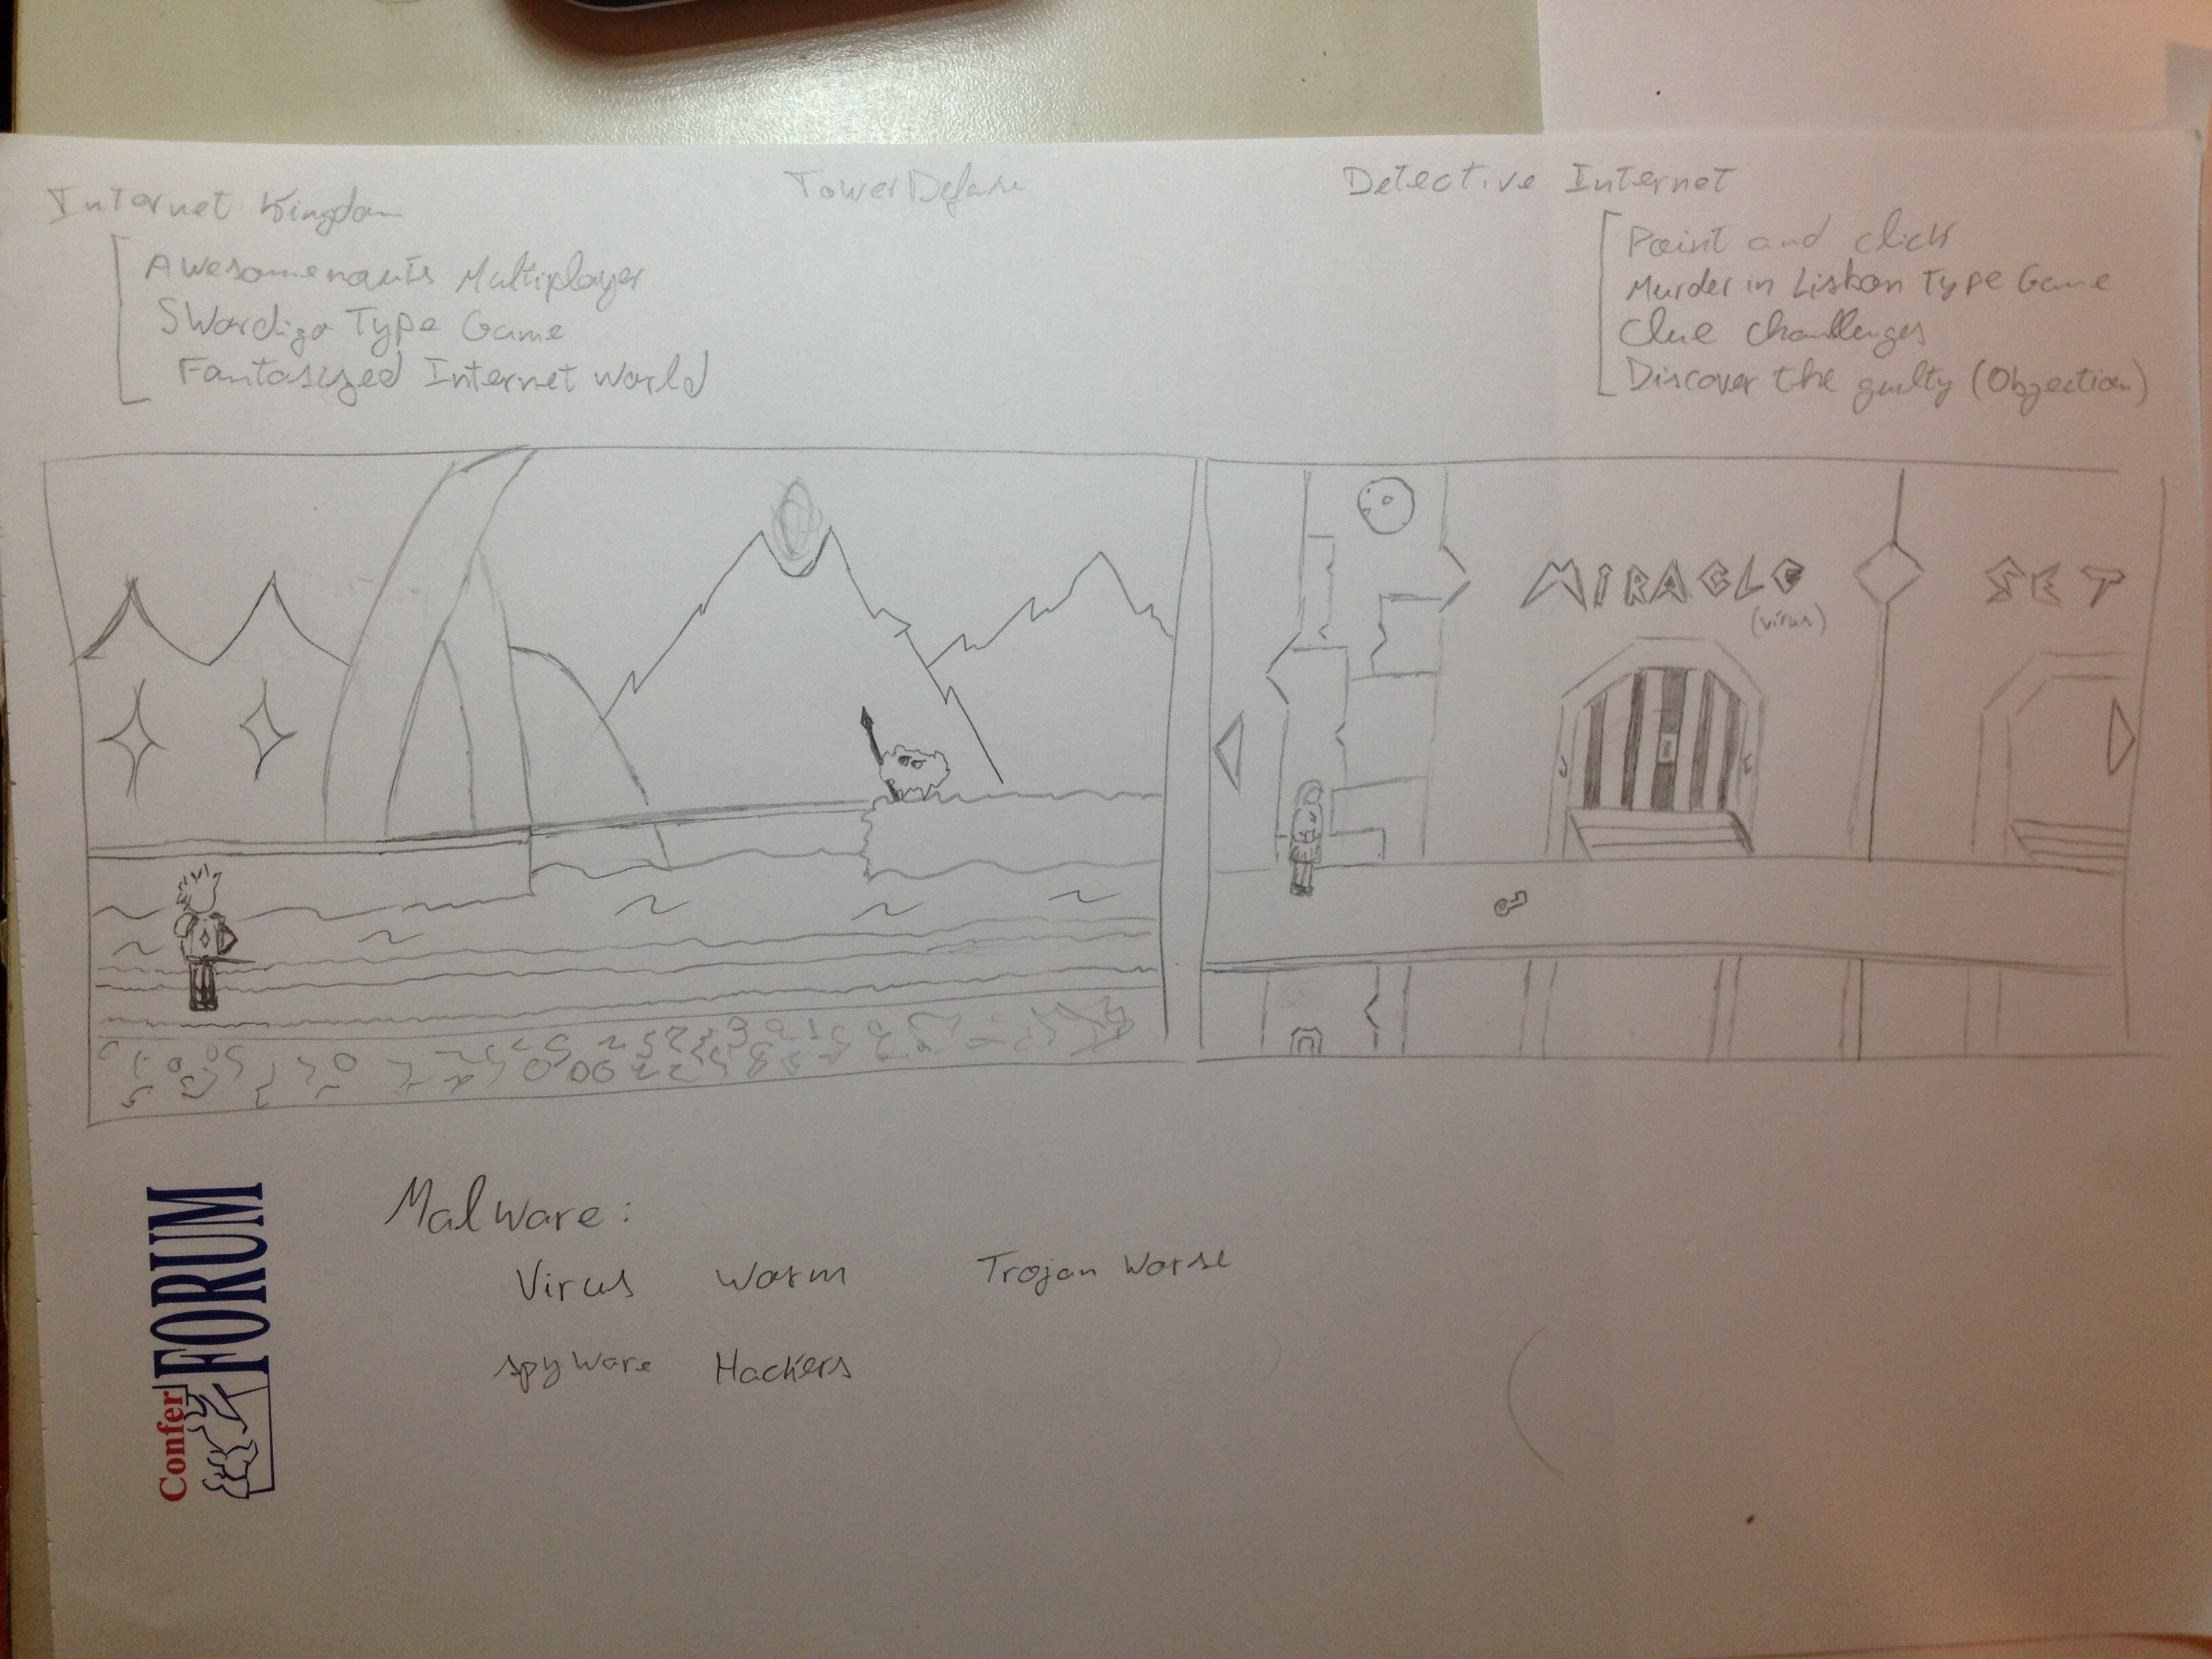
\includegraphics 
	[width = 0.75\textwidth] {Ricardo/ricardo_prototipo_1}
\caption{\label{fig:ric:prot1}} Protótipos do Ricardo
\end{figure}

Estes protótipos visavam jogos bastante diferentes. No lado esquerdo da Figura \ref{fig:ric:prot1} vemos um jogo ao estilo \textit{Hack and Slash}, o ideia por detrás deste jogo é que o jogador seria uma \textit{Ciber-Guardião} que defenderia a sua rede local de ataques de \textit{Malwares}, e a cada passo da história ir-se-ia descobrindo novos \textit{Malwares} e como nos proteger-mos deles.

Por sua vez, no lado direito da Figura \ref{fig:ric:prot1}, vemos um jogo de investigação, em que uma nova navegante da Internet teria de embarcar numa aventura para descobrir a entidade de um famoso \textit{Hacker}, que estava a destruir servidores e a espalhar medo pela Internet fora, e parar o seu reino de terror.
Ao longo do jogo, o jogador ia descobrindo os perigos dos \textit{Malwares} e como se proteger.

\subsection{Protótipos do Tiago}



\subsection{Protótipos do Ian}

O primeiro protótipo (Figura \ref{fig:ian:prot1}) foi um rail-shooter, onde se controlava uma nave, que transportava uma mensagem importante, e disparava caracteres de password. O objectivo seria levar a mensagem de um ponto a outro, protegendo-a de vários \textit{Vírus} e \textit{bosses} que iriam aparecendo ao longo dos níveis. Seria também possível apanhar \textit{power ups}, como escudos de Antivírus. Haveria dois modos, um modo campanha que seria uma série de níveis, e um modo infinito, que seria um nível que apenas acabaria quando o jogador ficasse sem vidas. Este modo infinito permitiria guardar a pontuação numa tabela para comparar com a de outros jogadores.

\begin{figure}[h]
\centering
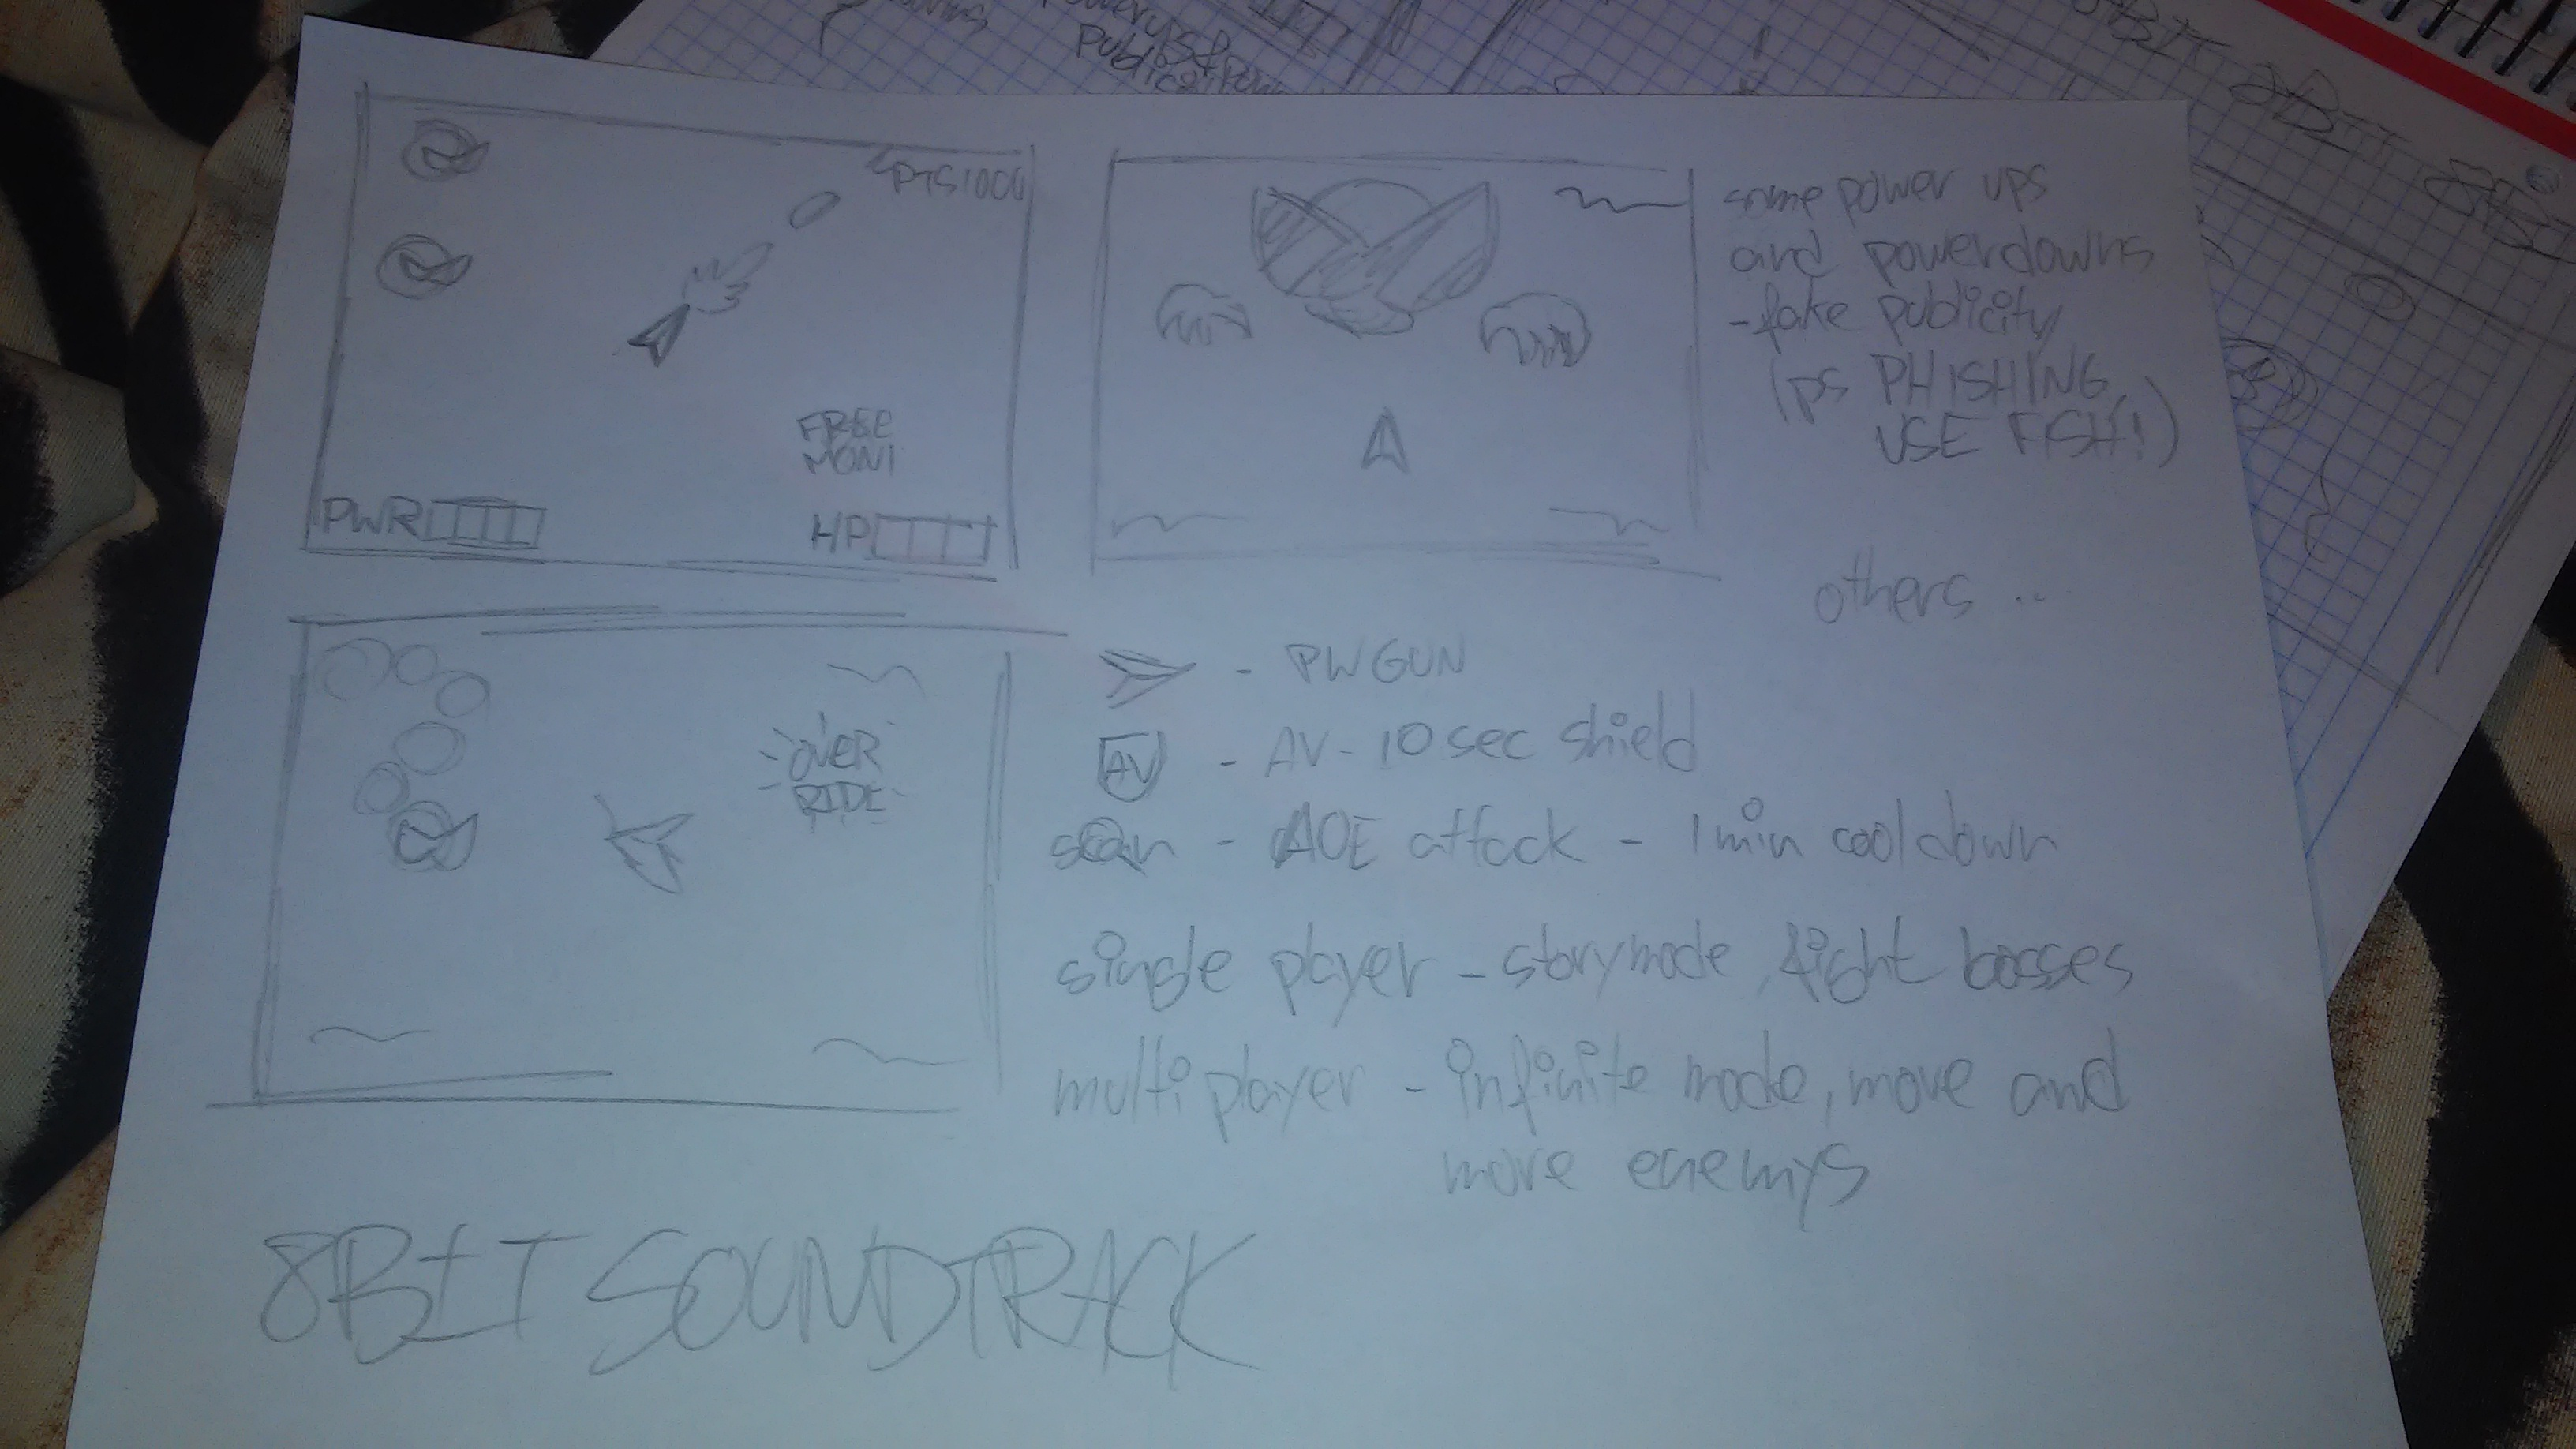
\includegraphics 
	[width = 0.75\textwidth] {Ian/ian_prototipo_1}
\caption{\label{fig:ian:prot1}} Primeiro Protótipo do Ian
\end{figure}

O segundo protótipo (Figura \ref{fig:ian:prot2}) era um \textit{God Game}, onde o jogador controlava um Deus das Nuvens (\textit{Clouds}). Esse Deus seria venerado inicialmente por uma vila, e o objectivo seria expandir essa vila, ganhando assim pontos. Com estes pontos seria possível desbloquear poderes, como por exemplo \textit{Firewalls} para proteger a vila de inimigos. Os inimigos poderiam ser vários tipo de vírus (\textit{Worms} seriam representados por serpentes gigantes, \textit{Trojans} cavalos, etc), ou outras vilas hostis, representando \textit{Hackers}. A movimentação dos habitantes pelas vilas seriam assim uma metáfora para a troca do informação pela \textit{Cloud}, e a expansão da vila o crescimento da \textit{Cloud}.

\begin{figure}[h]
\centering
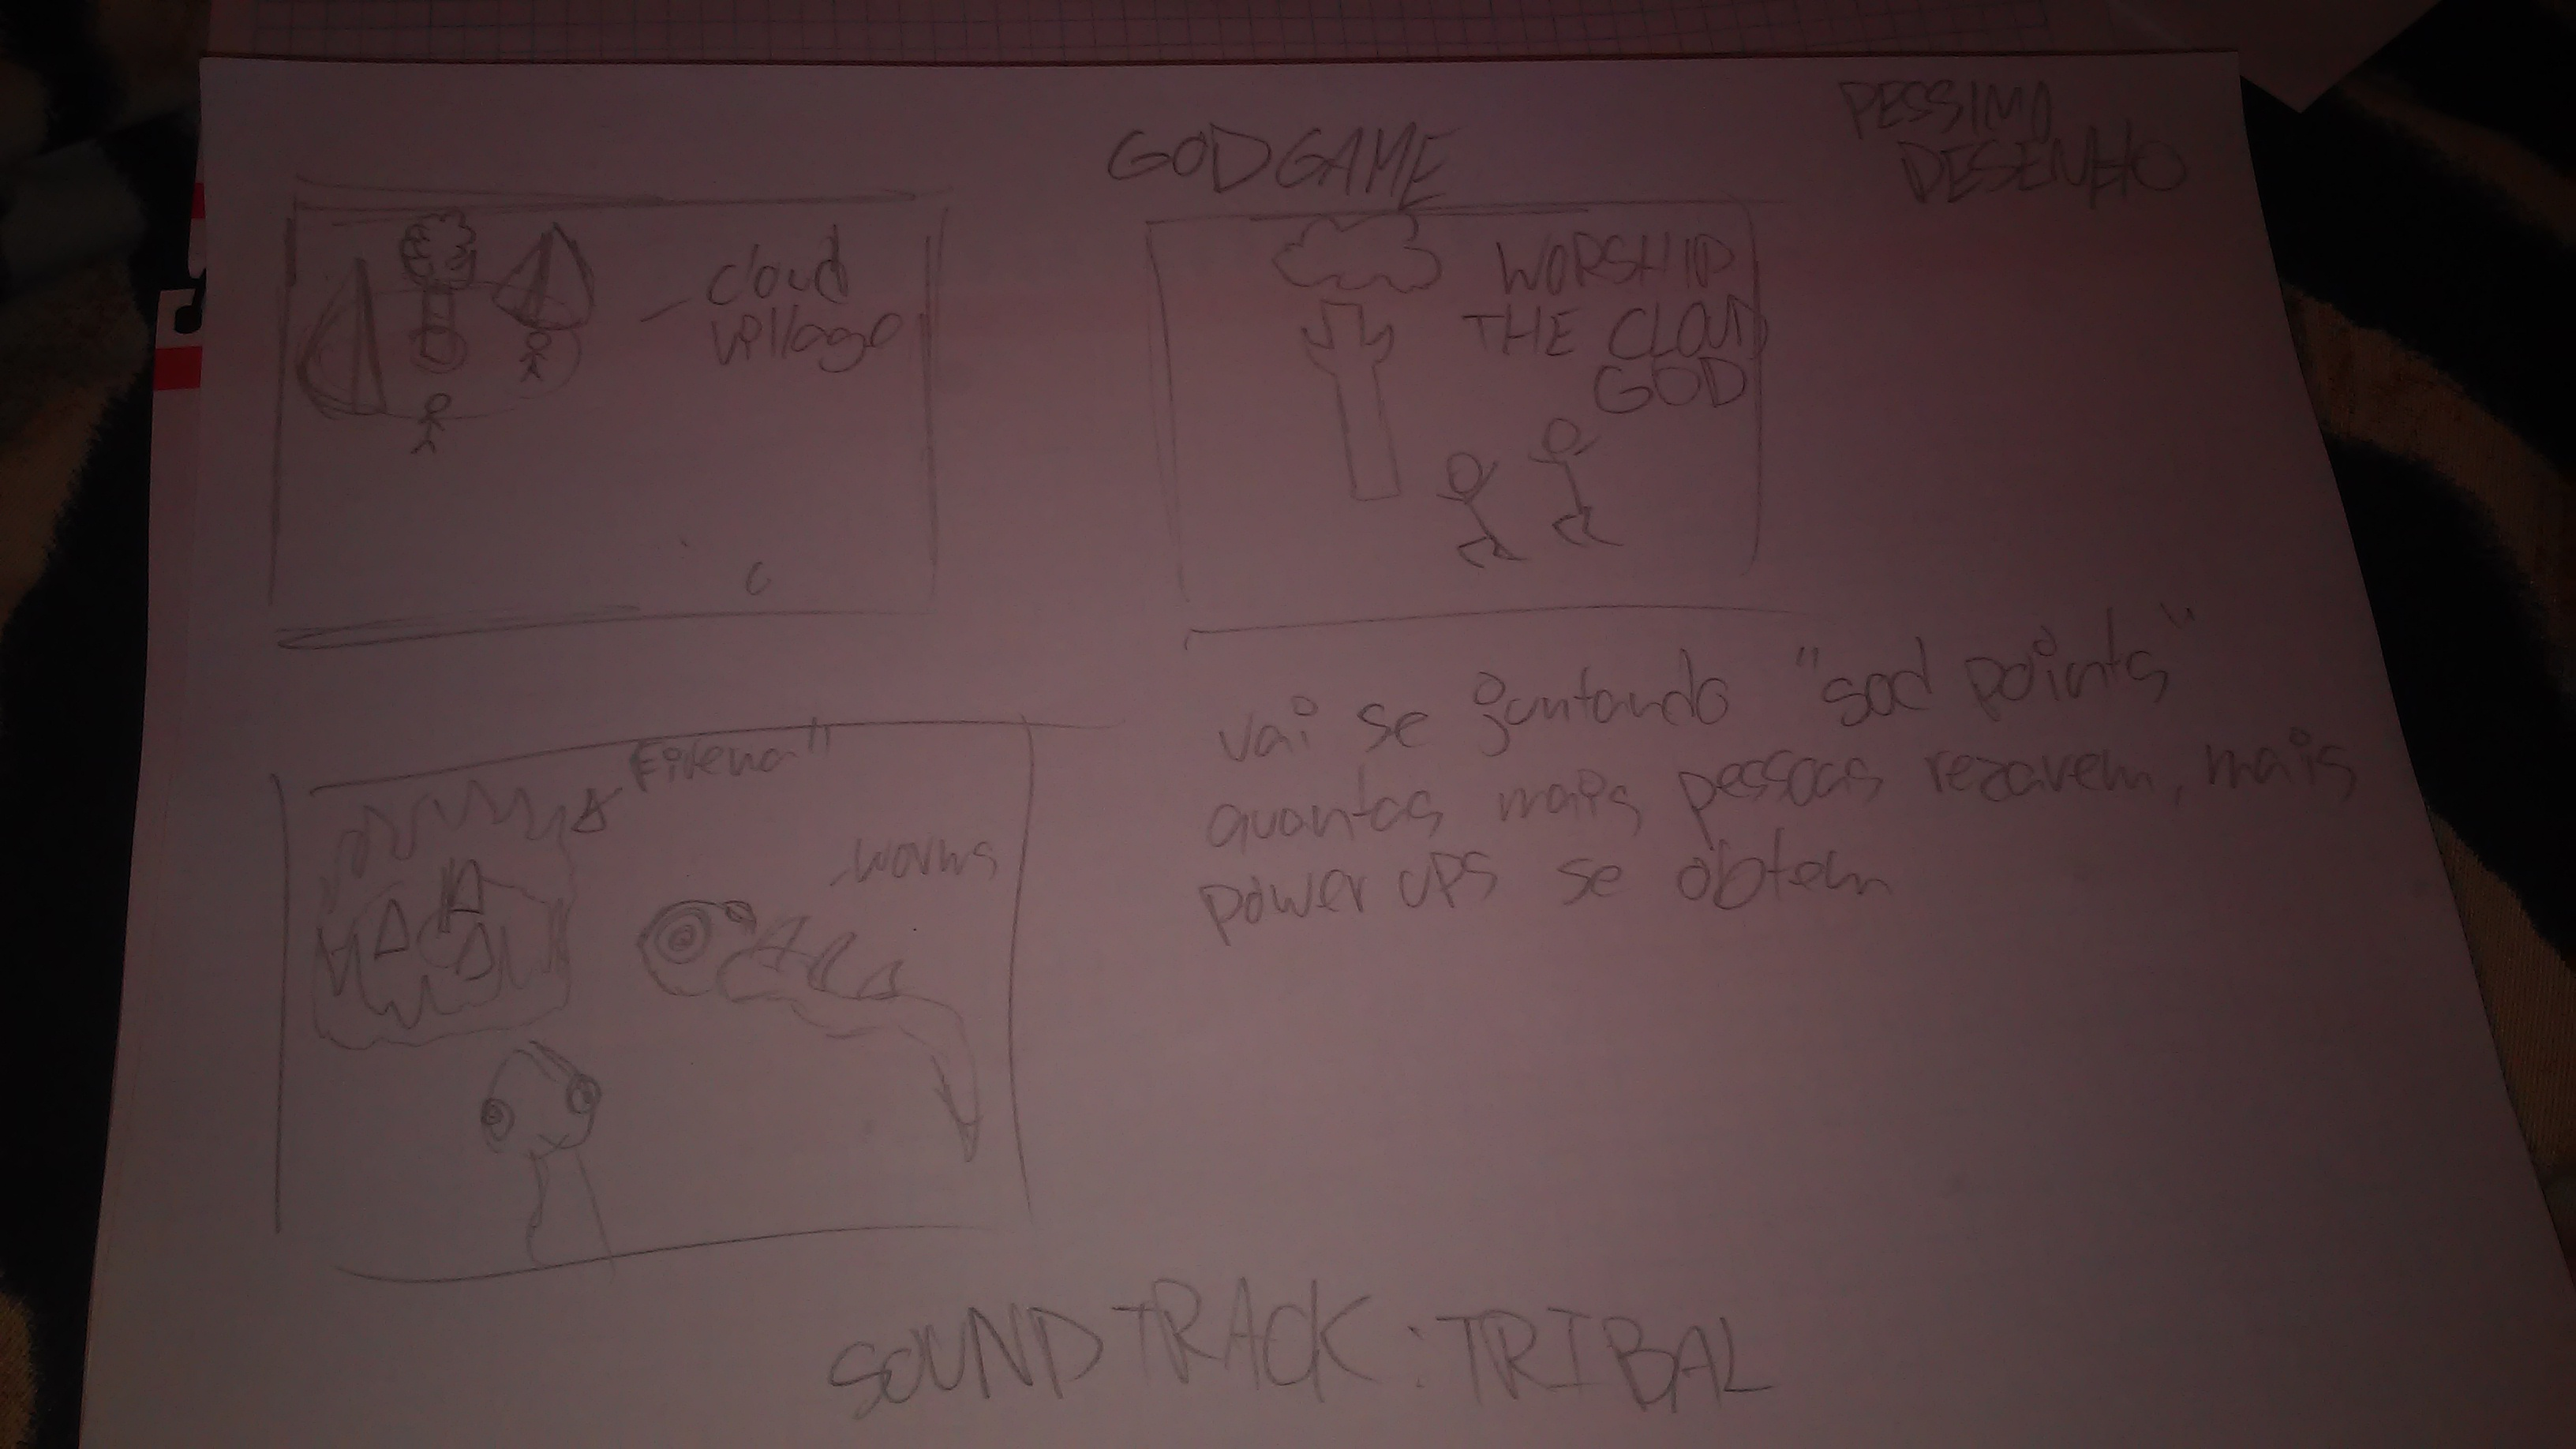
\includegraphics 
	[width = \textwidth] {Ian/ian_prototipo_2}
\caption{\label{fig:ian:prot2}} Segundo Protótipo do Ian
\end{figure}

\subsection{A Escolha}

Depois de cada elemento ter revelado os seus protótipos, foi feita uma escolha de qual deles seria usado para futuros passos, como a criação de um protótipo funcional.

Os protótipos que mais chamaram à atenção, pela sua criatividade e possíveis dinâmicas de jogo, foram o \textit{God Game}, que oferecia uma metáfora forte sobre a \textit{Cloud} e \textit{Malwares}, e o \textit{Hack and Slash}, que mostrava um jogo maior e mais complexo que implicava uma evolução da personagem e uma história forte. Infelizmente, por falta de conhecimentos para criar projectos assim tão grandes, decidiu-se optar por soluções mais pequenas.

Assim, as possíveis escolhas foram o \textit{Railshooter} e o \textit{Platformer}, quer

\section{Protótipos de Baixa Fidelidade}

Depois dos protótipos não-funcionais serem apresentados 

\chapter{Resultados dos Testes de Usabilidade}
\label{chap:results} 
%The results obtained from applying usability tests to all iterations/prototypes (showing the progress across iterations), including the final tests.


\chapter{Conclusão}
\label{chap:concl}
%Conclusions and suggestions for future work
Com este projecto tivemos a sorte de interagir com pessoas mais novas e com outras perspectivas do que é o mundo bastante diferente das nossas, o que nos obrigou a mudar a mentalidade para poder fazer algo que eles gostassem e que lhes passasse a mensagem.

Adicionalmente a criação dos inúmeros protótipos não-funcionais permitiu-nos ver o que \emph{podíamos} fazer e obrigou-nos a escolher algo que realmente \textbf{\emph{conseguíssemos}} fazer, sendo que as ideias que o grupo tinha mais interesse também eram as mais complexas.

Devido à ligação entre o grupo e a escola, é possível que o projecto não termine aquando do fim da disciplina de \ac{CCU}, permitindo assim um trabalho mais aprofundado com os alunos e facilitando a criação de um jogo completo.

\chapter{Anexos}


\section{Requesitos}
\label{att:requir}

Aqui apresentamos os requisitos criados como base para o nosso jogo.
É de notar que muitos requisitos foram modificados, adicionados ou eliminados à medida que o projecto foi sendo desenvolvido.

\begin{tabular} {|l|p{8cm}|} 
%\hline
%Item & Qty & Unit \\
\hline
Requisito \# & 1 \\
\hline
Tipo & Utilizador\\
\hline
Descrição & O sistema deve ser utilizado por alunos do secundário \\
\hline
Razão & Necessidade de passar a mensagem a um grupo de pessoas em idades vulneráveis a ataques informáticos. \\
\hline
Fonte & Ricardo Rodrigues \\
\hline
Critério de Avaliação & --- \\
\hline
Dependências & Nenhuma \\
\hline
História & Levantado por Ricardo Rodrigues, 2014/10/29 \\
\hline
\end{tabular}

\begin{tabular} {|l|p{8cm}|} 
%\hline
%Item & Qty & Unit \\
\hline
Requisito \# & 2 \\
\hline
Tipo & Ambiente \\
\hline
Descrição & O sistema deverá ser executado num browser \\
\hline
Razão & Os utilizadores desejam algo simples e que não exija muito tempo. \\
\hline
Fonte & Entrevistas \\
\hline
Critério de Avaliação & Executar o sistema num browser \\
\hline
Dependências & Nenhuma \\
\hline
História & Levantado por Tiago Martins, 2014/10/27 \\
\hline
\end{tabular}

\begin{tabular} {|l|p{8cm}|} 
%\hline
%Item & Qty & Unit \\
\hline
Requisito \# & 3 \\
\hline
Tipo & Ambiente \\
\hline
Descrição & Para executar o sistema é necessário um computador com acesso à internet \\
\hline
Razão & A maior parte do grupo de foco tem acesso a esta plataforma e torna o acesso ao sistema mais fácil de partilhar. \\
\hline
Fonte & Entrevistas \\
\hline
Critério de Avaliação & Executar o sistema num browser apenas com acesso à internet\\
\hline
Dependências & Nenhuma \\
\hline
História & Levantado por Tiago Martins, 2014/10/27 \\
\hline
\end{tabular}

\begin{tabular} {|l|p{8cm}|} 
%\hline
%Item & Qty & Unit \\
\hline
Requisito \# & 4 \\
\hline
Tipo & Funcional \\
\hline
Descrição & O sistema deve mostrar os perigos da internet. \\
\hline
Razão & A necessidade dos utilizadores de ficarem com uma noção de que perigos correm quando visitam a internet. \\
\hline
Fonte & Objectivo do Projecto \\
\hline
Critério de Avaliação & Nenhum\\
\hline
Dependências & 5, 6 e 7 \\
\hline
História & Levantado por Ricardo Rodrigues, 2014/11/03 \\
\hline
\end{tabular}

\begin{tabular} {|l|p{8cm}|} 
%\hline
%Item & Qty & Unit \\
\hline
Requisito \# & 5 \\
\hline
Tipo & Funcional \\
\hline
Descrição & O sistema deve mostrar o que é um vírus informático. \\
\hline
Razão & A necessidade dos utilizadores de ficarem com uma noção de que perigos correm quando visitam a internet. \\
\hline
Fonte & Objectivo do Projecto \\
\hline
Critério de Avaliação & Nenhum\\
\hline
Dependências & Nenhuma \\
\hline
História & Levantado por Ricardo Rodrigues, 2014/11/11 \\
\hline
\end{tabular}

\begin{tabular} {|l|p{8cm}|} 
%\hline
%Item & Qty & Unit \\
\hline
Requisito \# & 6 \\
\hline
Tipo & Funcional \\
\hline
Descrição & O sistema deve mostrar o que é um Spyware. \\
\hline
Razão & A necessidade dos utilizadores de ficarem com uma noção de que perigos correm quando visitam a internet. \\
\hline
Fonte & Objectivo do Projecto \\
\hline
Critério de Avaliação & Nenhum\\
\hline
Dependências & Nenhuma \\
\hline
História & Levantado por Ricardo Rodrigues, 2014/11/11 \\
\hline
\end{tabular}

\begin{tabular} {|l|p{8cm}|} 
%\hline
%Item & Qty & Unit \\
\hline
Requisito \# & 7 \\
\hline
Tipo & Funcional \\
\hline
Descrição & O sistema deve mostrar o que é um Hacker. \\
\hline
Razão & A necessidade dos utilizadores de ficarem com uma noção de que perigos correm quando visitam a internet. \\
\hline
Fonte & Objectivo do Projecto \\
\hline
Critério de Avaliação & Nenhum\\
\hline
Dependências & Nenhuma \\
\hline
História & Levantado por Ricardo Rodrigues, 2014/11/11 \\
\hline
\end{tabular}

\begin{tabular} {|l|p{8cm}|} 
%\hline
%Item & Qty & Unit \\
\hline
Requisito \# & 8 \\
\hline
Tipo & Funcional \\
\hline
Descrição & O sistema deve mostrar como os utilizadores se podem proteger dos perigos da internet. \\
\hline
Razão & A necessidade dos utilizadores de ficarem com uma noção de que perigos correm quando visitam a internet e como se proteger. \\
\hline
Fonte & Objectivo do Projecto \\
\hline
Critério de Avaliação & Nenhum\\
\hline
Dependências & 9, 10 e 11 \\
\hline
História & Levantado por Ricardo Rodrigues, 2014/11/03 \\
\hline
\end{tabular}

\begin{tabular} {|l|p{8cm}|} 
%\hline
%Item & Qty & Unit \\
\hline
Requisito \# & 9 \\
\hline
Tipo & Funcional \\
\hline
Descrição & O sistema deve mostrar o que é um Anti-Vírus. \\
\hline
Razão & A necessidade dos utilizadores de ficarem com uma noção de que perigos correm quando visitam a internet e como se proteger. \\
\hline
Fonte & Objectivo do Projecto \\
\hline
Critério de Avaliação & Nenhum\\
\hline
Dependências & Nenhuma \\
\hline
História & Levantado por Ricardo Rodrigues, 2014/11/11 \\
\hline
\end{tabular}

\begin{tabular} {|l|p{8cm}|} 
%\hline
%Item & Qty & Unit \\
\hline
Requisito \# & 10 \\
\hline
Tipo & Funcional \\
\hline
Descrição & O sistema deve mostrar o que é um Anti-Spyware. \\
\hline
Razão & A necessidade dos utilizadores de ficarem com uma noção de que perigos correm quando visitam a internet e como se proteger. \\
\hline
Fonte & Objectivo do Projecto \\
\hline
Critério de Avaliação & Nenhum\\
\hline
Dependências & Nenhuma \\
\hline
História & Levantado por Ricardo Rodrigues, 2014/11/11 \\
\hline
\end{tabular}

\begin{tabular} {|l|p{8cm}|} 
%\hline
%Item & Qty & Unit \\
\hline
Requisito \# & 11 \\
\hline
Tipo & Funcional \\
\hline
Descrição & O sistema deve mostrar ao utilizador que deve fazer updates regulares ao sistema e ao software de protecção. \\
\hline
Razão & A necessidade dos utilizadores de ficarem com uma noção de que perigos correm quando visitam a internet e como se proteger. \\
\hline
Fonte & Objectivo do Projecto \\
\hline
Critério de Avaliação & Nenhum\\
\hline
Dependências & Nenhuma \\
\hline
História & Levantado por Ricardo Rodrigues, 2014/11/11 \\
\hline
\end{tabular}

\begin{tabular} {|l|p{8cm}|} 
%\hline
%Item & Qty & Unit \\
\hline
Requisito \# & 12 \\
\hline
Tipo & Funcional \\
\hline
Descrição & O utilizador deve poder escolher o modo Campanha. \\
\hline
Razão & Necessidade dos utilizadores de terem uma história envolvente. \\
\hline
Fonte & Entrevista \\
\hline
Critério de Avaliação & O sistema terá um modo de campanha. \\
\hline
Dependências & 13 e 14 \\
\hline
História & Levantado por Tiago Martins e Ricardo Rodrigues, 2014/10/29 \\
\hline
\end{tabular}

\begin{tabular} {|l|p{8cm}|} 
%\hline
%Item & Qty & Unit \\
\hline
Requisito \# & 13 \\
\hline
Tipo & Funcional \\
\hline
Descrição & O modo Campanha é composto por níveis. \\
\hline
Razão & Os utilizadores podem querer voltar a refazer o nível. \\
\hline
Fonte & Entrevista \\
\hline
Critério de Avaliação & O sistema terá um modo de campanha. \\
\hline
Dependências & 14 \\
\hline
História & Levantado por Ricardo Rodrigues, 2014/11/11 \\
\hline
\end{tabular}

\begin{tabular} {|l|p{8cm}|} 
%\hline
%Item & Qty & Unit \\
\hline
Requisito \# & 14 \\
\hline
Tipo & Funcional \\
\hline
Descrição & Cada nível tem uma pontuação. \\
\hline
Razão & Necessidade dos utilizadores compararem resultados. \\
\hline
Fonte & Entrevistas \\
\hline
Critério de Avaliação & Nenhum \\
\hline
Dependências & Nenhuma \\
\hline
História & Levantado por Ricardo Rodrigues, 2014/11/11 \\
\hline
\end{tabular}

\begin{tabular} {|l|p{8cm}|} 
%\hline
%Item & Qty & Unit \\
\hline
Requisito \# & 15 \\
\hline
Tipo & Funcional \\
\hline
Descrição & Cada inimigo derrotado aumenta a pontuação do nível. \\
\hline
Razão & Necessidade dos utilizadores compararem resultados. \\
\hline
Fonte & Entrevistas \\
\hline
Critério de Avaliação & Nenhum \\
\hline
Dependências & 16, 17 e 18 \\
\hline
História & Levantado por Ricardo Rodrigues, 2014/11/19 \\
\hline
\end{tabular}

\begin{tabular} {|l|p{8cm}|} 
%\hline
%Item & Qty & Unit \\
\hline
Requisito \# & 16 \\
\hline
Tipo & Funcional \\
\hline
Descrição & Os vírus aumentam a pontuação do nível em 20 pontos \\
\hline
Razão & Necessidade dos utilizadores compararem resultados. \\
\hline
Fonte & Entrevistas \\
\hline
Critério de Avaliação & Nenhum \\
\hline
Dependências & Nenhuma \\
\hline
História & Levantado por Ricardo Rodrigues, 2014/11/19 \\
\hline
\end{tabular}

\begin{tabular} {|l|p{8cm}|} 
%\hline
%Item & Qty & Unit \\
\hline
Requisito \# & 17 \\
\hline
Tipo & Funcional \\
\hline
Descrição & Os hackers aumentam a pontuação do nível em 5000 pontos \\
\hline
Razão & Necessidade dos utilizadores compararem resultados. \\
\hline
Fonte & Entrevistas \\
\hline
Critério de Avaliação & Nenhum \\
\hline
Dependências & Nenhuma \\
\hline
História & Levantado por Ricardo Rodrigues, 2014/11/19 \\
\hline
\end{tabular}

\begin{tabular} {|l|p{8cm}|} 
%\hline
%Item & Qty & Unit \\
\hline
Requisito \# & 18 \\
\hline
Tipo & Funcional \\
\hline
Descrição & Os Spywares aumentam a pontuação do nível em 40 pontos \\
\hline
Razão & Necessidade dos utilizadores compararem resultados. \\
\hline
Fonte & Entrevistas \\
\hline
Critério de Avaliação & Nenhum \\
\hline
Dependências & Nenhuma \\
\hline
História & Levantado por Ricardo Rodrigues, 2014/11/19 \\
\hline
\end{tabular}

\begin{tabular} {|l|p{8cm}|} 
%\hline
%Item & Qty & Unit \\
\hline
Requisito \# & 19 \\
\hline
Tipo & Funcional \\
\hline
Descrição & O jogador tem três vidas. \\
\hline
Razão & Necessidade do utilizador verificar o estado do jogo \\
\hline
Fonte & Nenhuma \\
\hline
Critério de Avaliação & Nenhum \\
\hline
Dependências & 20, 21 e 22 \\
\hline
História & Levantado por Ricardo Rodrigues e Tiago Martins, 2014/11/24 \\
\hline
\end{tabular}

\begin{tabular} {|l|p{8cm}|} 
%\hline
%Item & Qty & Unit \\
\hline
Requisito \# & 20 \\
\hline
Tipo & Funcional \\
\hline
Descrição & Sempre que o jogador é atingido por um malware perde uma vida \\
\hline
Razão & Necessidade do utilizador verificar o estado do jogo \\
\hline
Fonte & Nenhuma \\
\hline
Critério de Avaliação & Nenhum \\
\hline
Dependências & Nenhuma \\
\hline
História & Levantado por Ricardo Rodrigues e Tiago Martins, 2014/11/24 \\
\hline
\end{tabular}

\begin{tabular} {|l|p{8cm}|} 
%\hline
%Item & Qty & Unit \\
\hline
Requisito \# & 21 \\
\hline
Tipo & Funcional \\
\hline
Descrição & Sempre que o jogador é atingido por uma bala perde uma vida \\
\hline
Razão & Necessidade do utilizador verificar o estado do jogo \\
\hline
Fonte & Nenhuma \\
\hline
Critério de Avaliação & Nenhum \\
\hline
Dependências & Nenhuma \\
\hline
História & Levantado por Ricardo Rodrigues, 2015/1/8 \\
\hline
\end{tabular}

\begin{tabular} {|l|p{8cm}|} 
%\hline
%Item & Qty & Unit \\
\hline
Requisito \# & 22 \\
\hline
Tipo & Funcional \\
\hline
Descrição & Quando o jogador perde as três vidas o jogo termina \\
\hline
Razão & Necessidade do utilizador verificar o estado do jogo \\
\hline
Fonte & Nenhuma \\
\hline
Critério de Avaliação & Nenhum \\
\hline
Dependências & Nenhuma \\
\hline
História & Levantado por Ricardo Rodrigues e Tiago Martins, 2014/11/24 \\
\hline
\end{tabular}

\begin{tabular} {|l|p{8cm}|} 
%\hline
%Item & Qty & Unit \\
\hline
Requisito \# & 23 \\
\hline
Tipo & Funcional \\
\hline
Descrição & Quando o jogador perde as três vidas o jogo termina \\
\hline
Razão & Necessidade do utilizador verificar o estado do jogo \\
\hline
Fonte & Nenhuma \\
\hline
Critério de Avaliação & Nenhum \\
\hline
Dependências & Nenhuma \\
\hline
História & Levantado por Ricardo Rodrigues e Tiago Martins, 2014/11/24 \\
\hline
\end{tabular}

\begin{tabular} {|l|p{8cm}|} 
%\hline
%Item & Qty & Unit \\
\hline
Requisito \# & 24 \\
\hline
Tipo & Funcional \\
\hline
Descrição & Quando um malware é atingido perde uma vida \\
\hline
Razão & Necessidade do utilizador verificar o estado do jogo \\
\hline
Fonte & Nenhuma \\
\hline
Critério de Avaliação & Nenhum \\
\hline
Dependências & 25, 26 e 27 \\
\hline
História & Levantado por Ricardo Rodrigues e Tiago Martins, 2014/11/24 \\
\hline
\end{tabular}

\begin{tabular} {|l|p{8cm}|} 
%\hline
%Item & Qty & Unit \\
\hline
Requisito \# & 25 \\
\hline
Tipo & Funcional \\
\hline
Descrição & Um vírus tem uma vida \\
\hline
Razão & Necessidade do utilizador verificar o estado do jogo \\
\hline
Fonte & Nenhuma \\
\hline
Critério de Avaliação & Nenhum \\
\hline
Dependências & Nenhuma \\
\hline
História & Levantado por Ricardo Rodrigues e Tiago Martins, 2014/11/24 \\
\hline
\end{tabular}

\begin{tabular} {|l|p{8cm}|} 
%\hline
%Item & Qty & Unit \\
\hline
Requisito \# & 26 \\
\hline
Tipo & Funcional \\
\hline
Descrição & Um Spyware tem 2 vidas \\
\hline
Razão & Necessidade do utilizador verificar o estado do jogo \\
\hline
Fonte & Nenhuma \\
\hline
Critério de Avaliação & Nenhum \\
\hline
Dependências & Nenhuma \\
\hline
História & Levantado por Ricardo Rodrigues e Tiago Martins, 2014/1/8 \\
\hline
\end{tabular}

\begin{tabular} {|l|p{8cm}|} 
%\hline
%Item & Qty & Unit \\
\hline
Requisito \# & 27 \\
\hline
Tipo & Funcional \\
\hline
Descrição & Um Hacker tem 5 vidas \\
\hline
Razão & Necessidade do utilizador verificar o estado do jogo \\
\hline
Fonte & Nenhuma \\
\hline
Critério de Avaliação & Nenhum \\
\hline
Dependências & Nenhuma \\
\hline
História & Levantado por Ricardo Rodrigues e Tiago Martins, 2014/1/8 \\
\hline
\end{tabular}

\section{Protótipos}
\label{att:proto}

\begin{figure}[h]
\centering
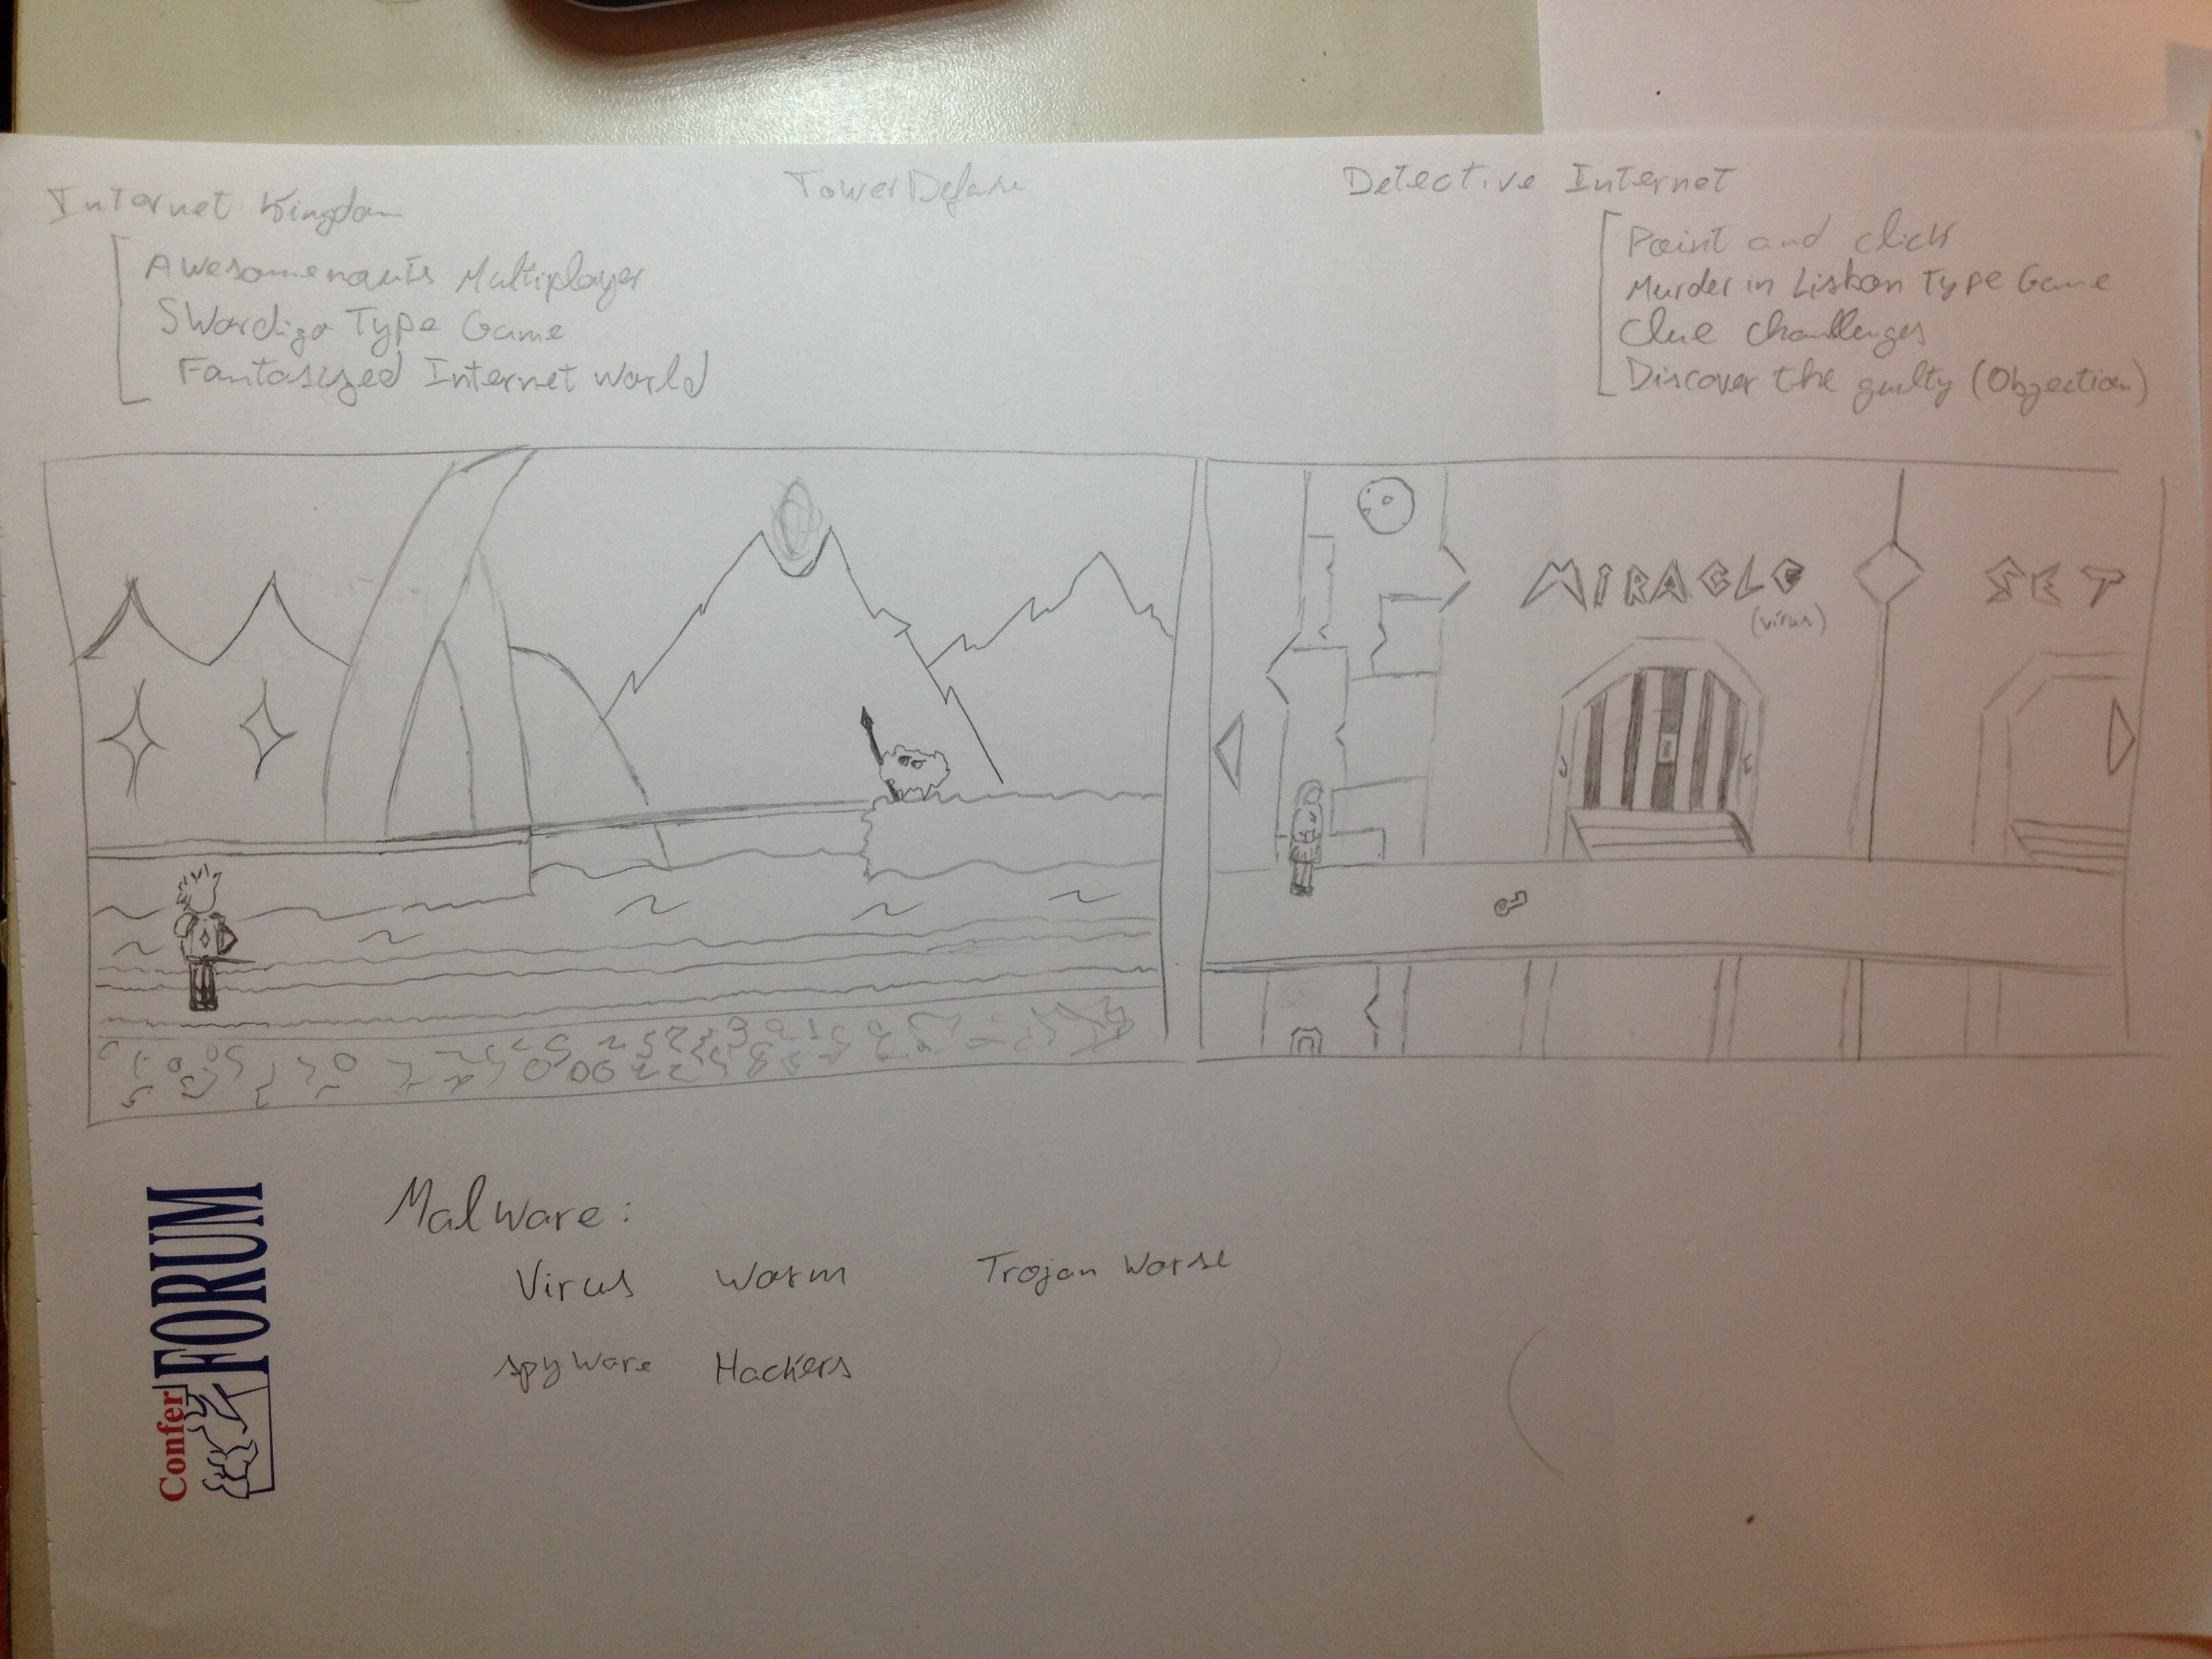
\includegraphics 
	[width = 0.75\textwidth] {Ricardo/ricardo_prototipo_1}
\caption{\label{att:fig:ric:prot1}} Primeiro Protótipo do Ricardo
\end{figure}

\begin{figure}[h]
\centering
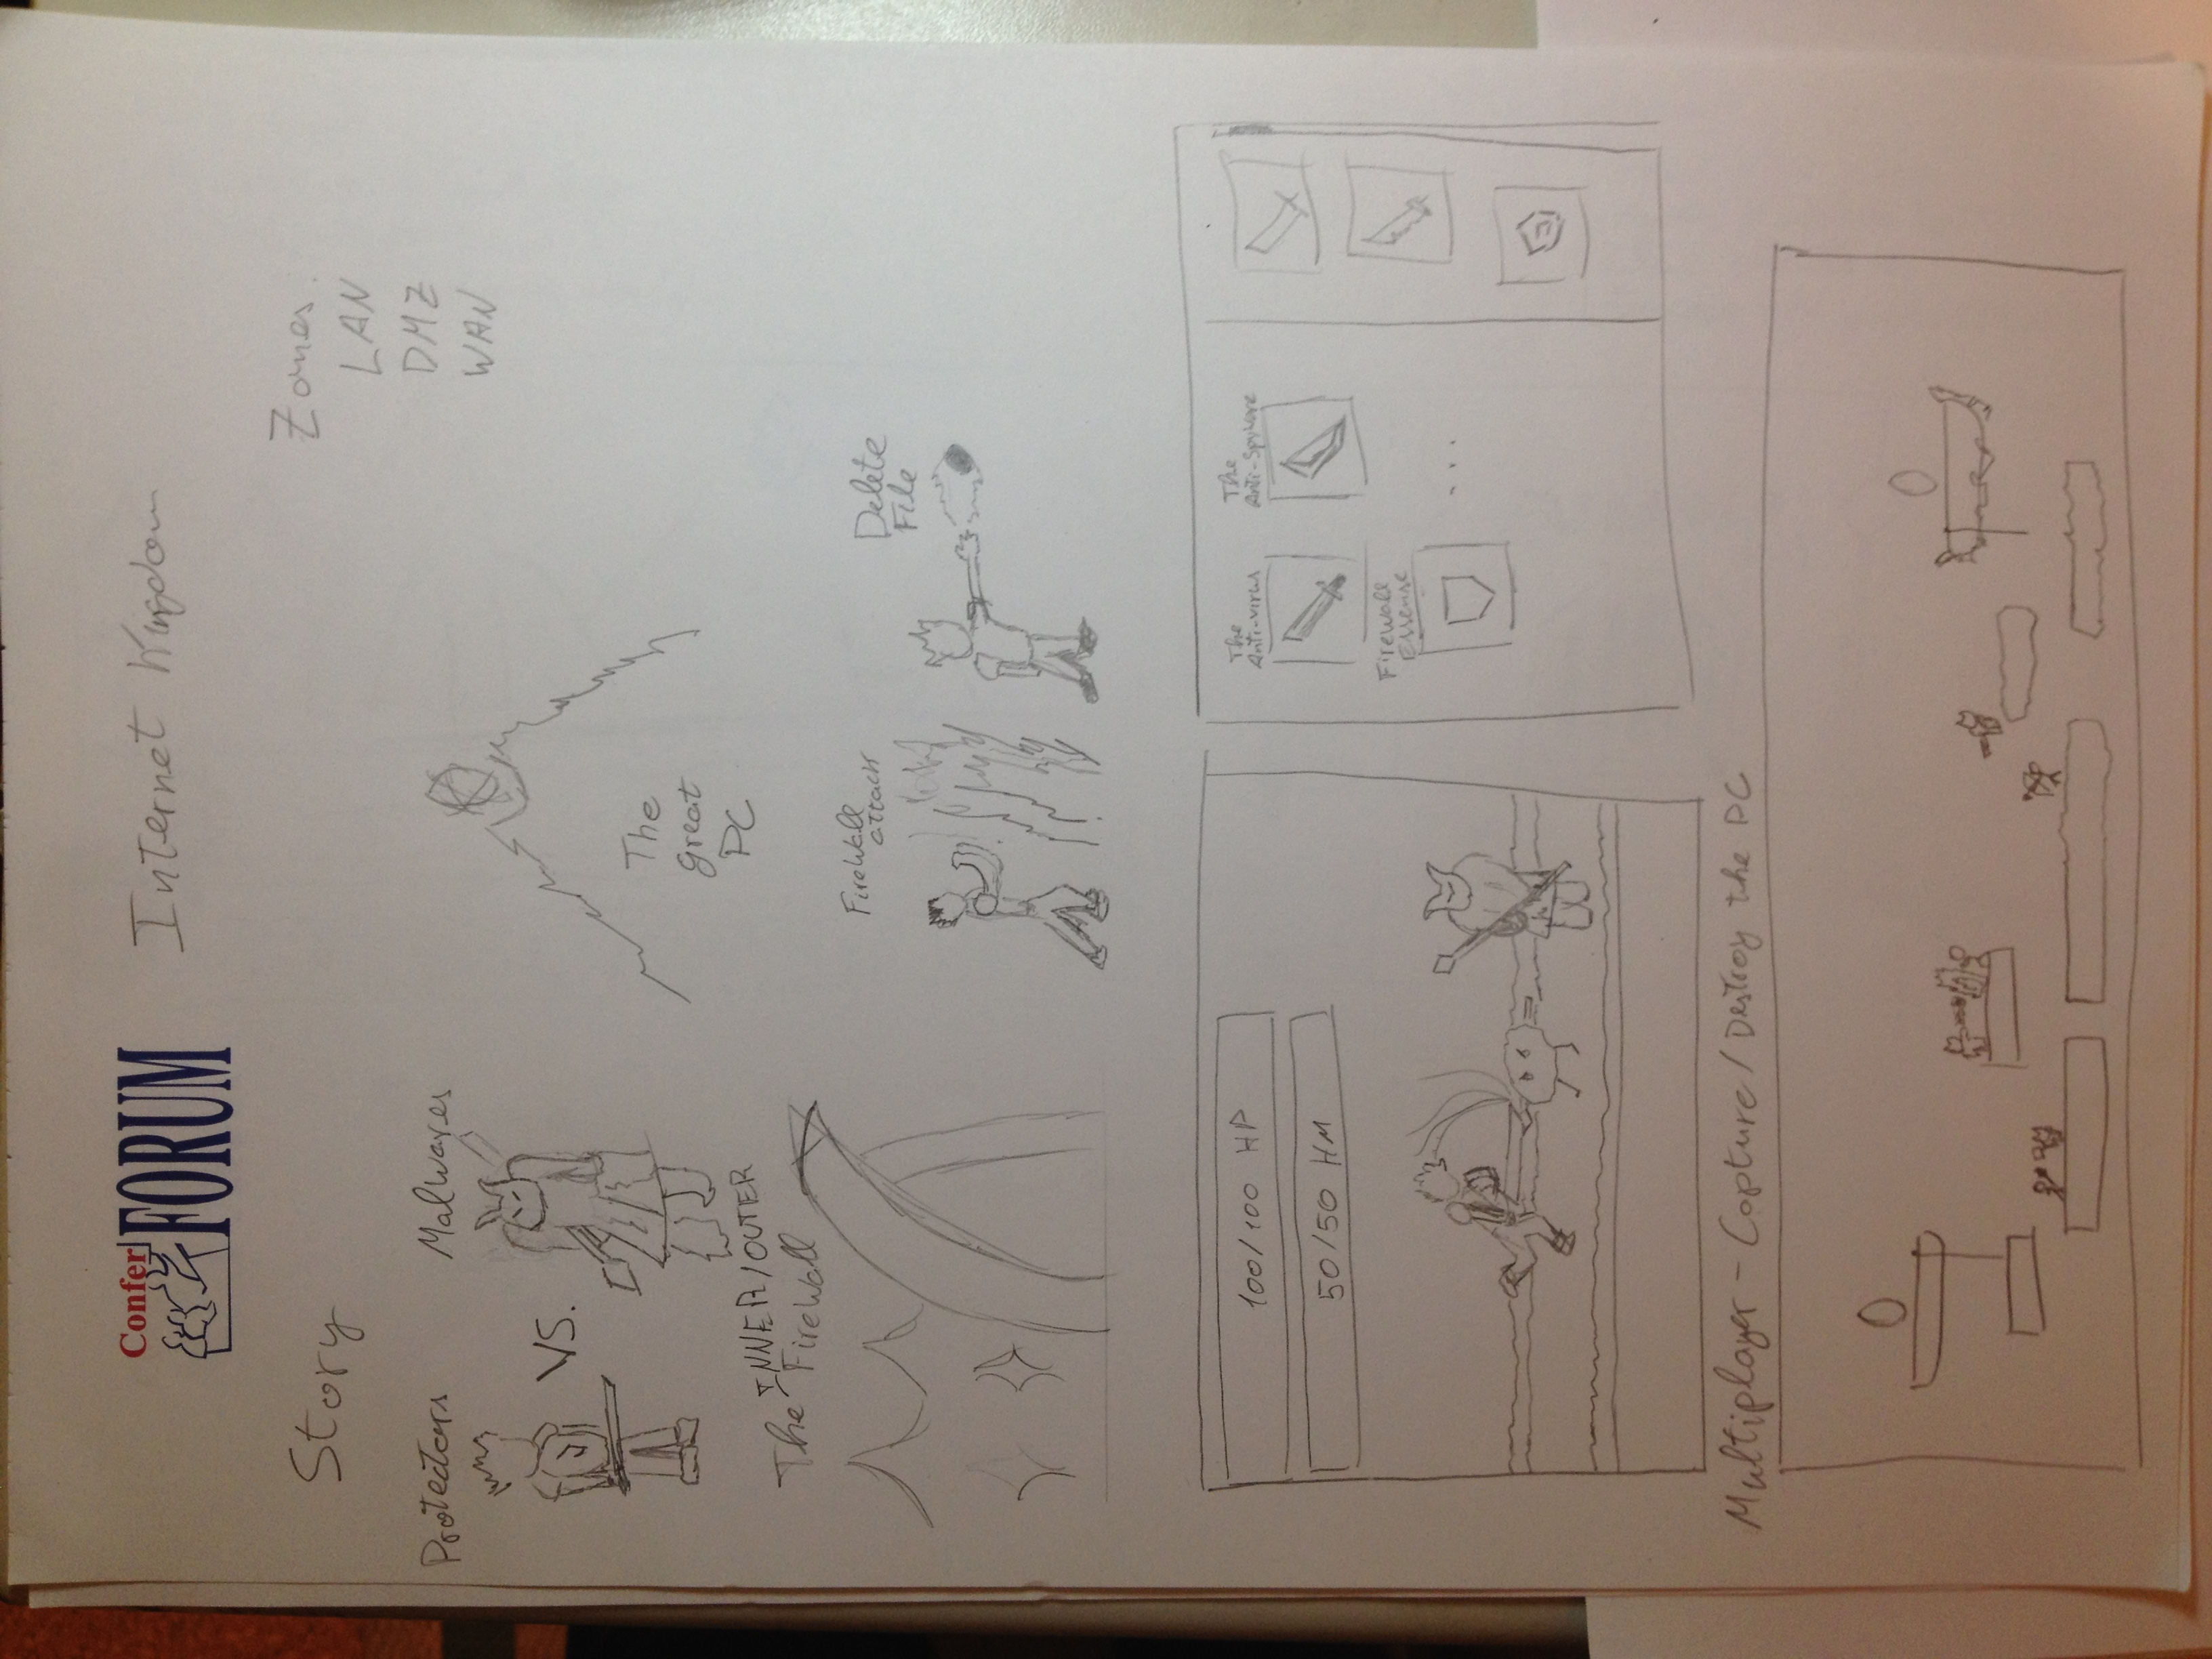
\includegraphics 
	[width = 0.75\textwidth , angle = 270] {Ricardo/ricardo_prototipo_2}
\caption{\label{att:fig:ric:prot2}} Segundo Protótipo do Ricardo
\end{figure}

\begin{figure}[h]
\centering
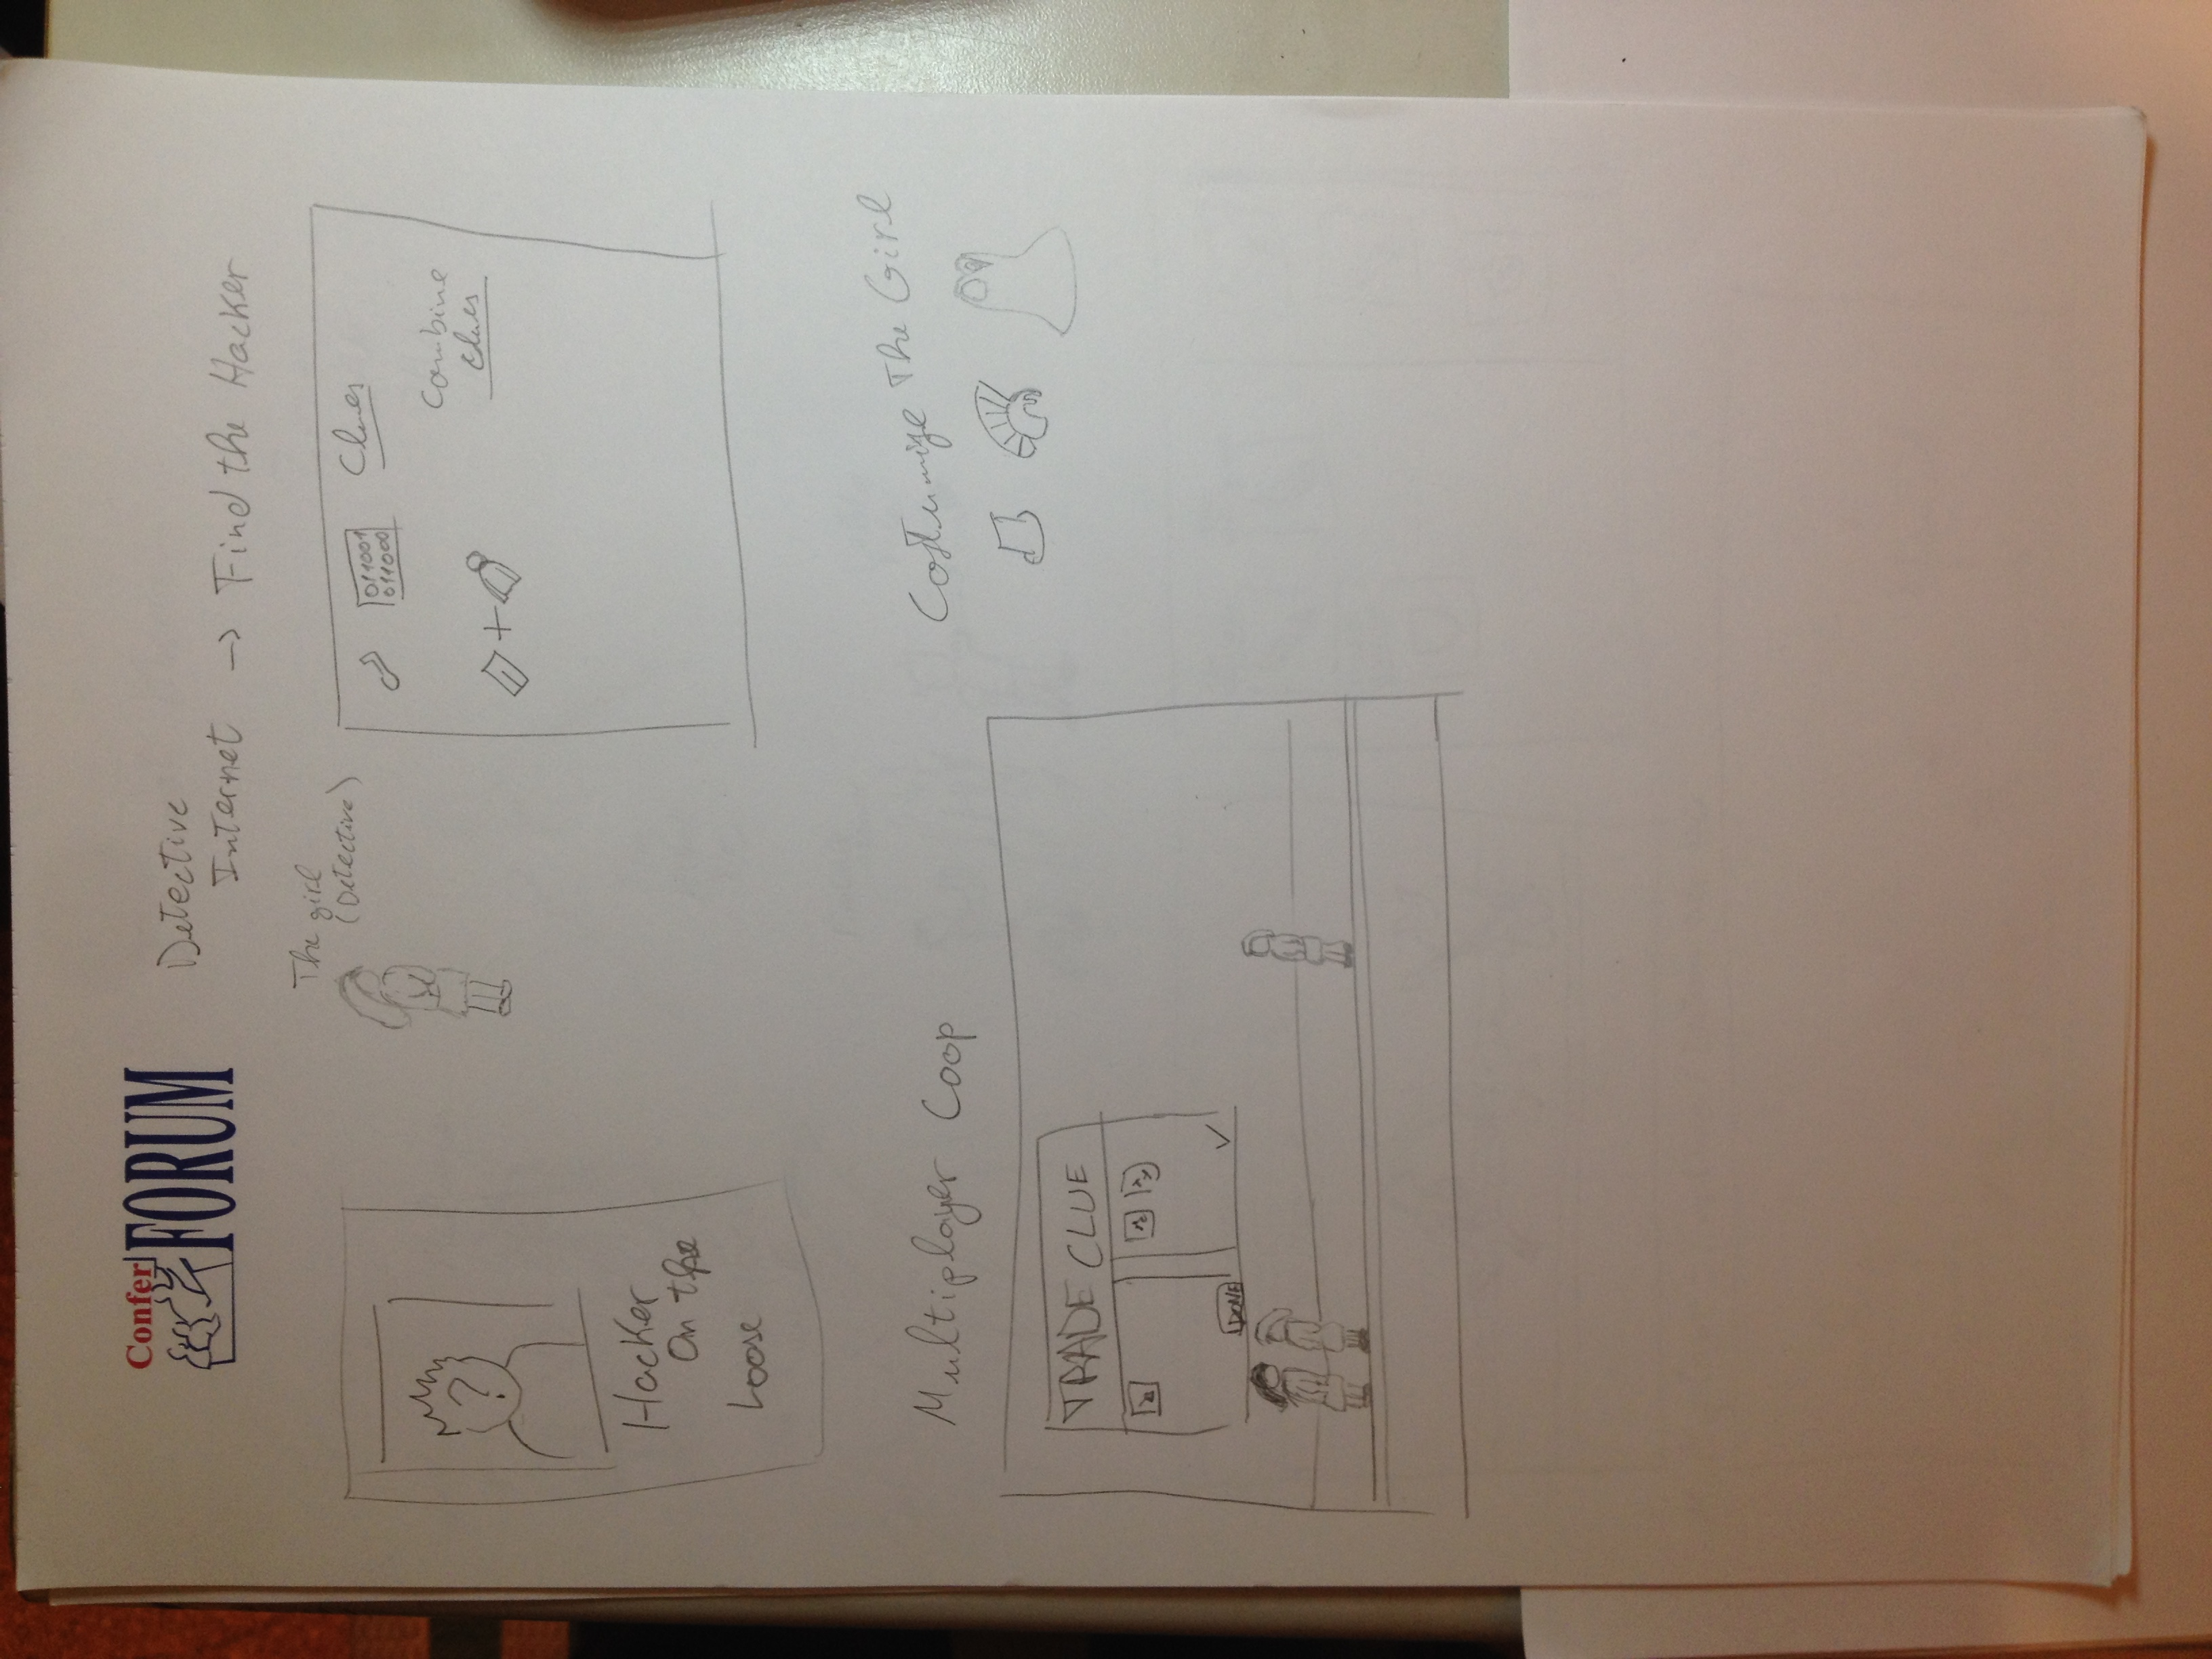
\includegraphics 
	[width = 0.75\textwidth , angle = 270] {Ricardo/ricardo_prototipo_3}
\caption{\label{att:fig:ric:prot3}} TerceiroProtótipo do Ricardo
\end{figure}

\begin{figure}[h]
\centering
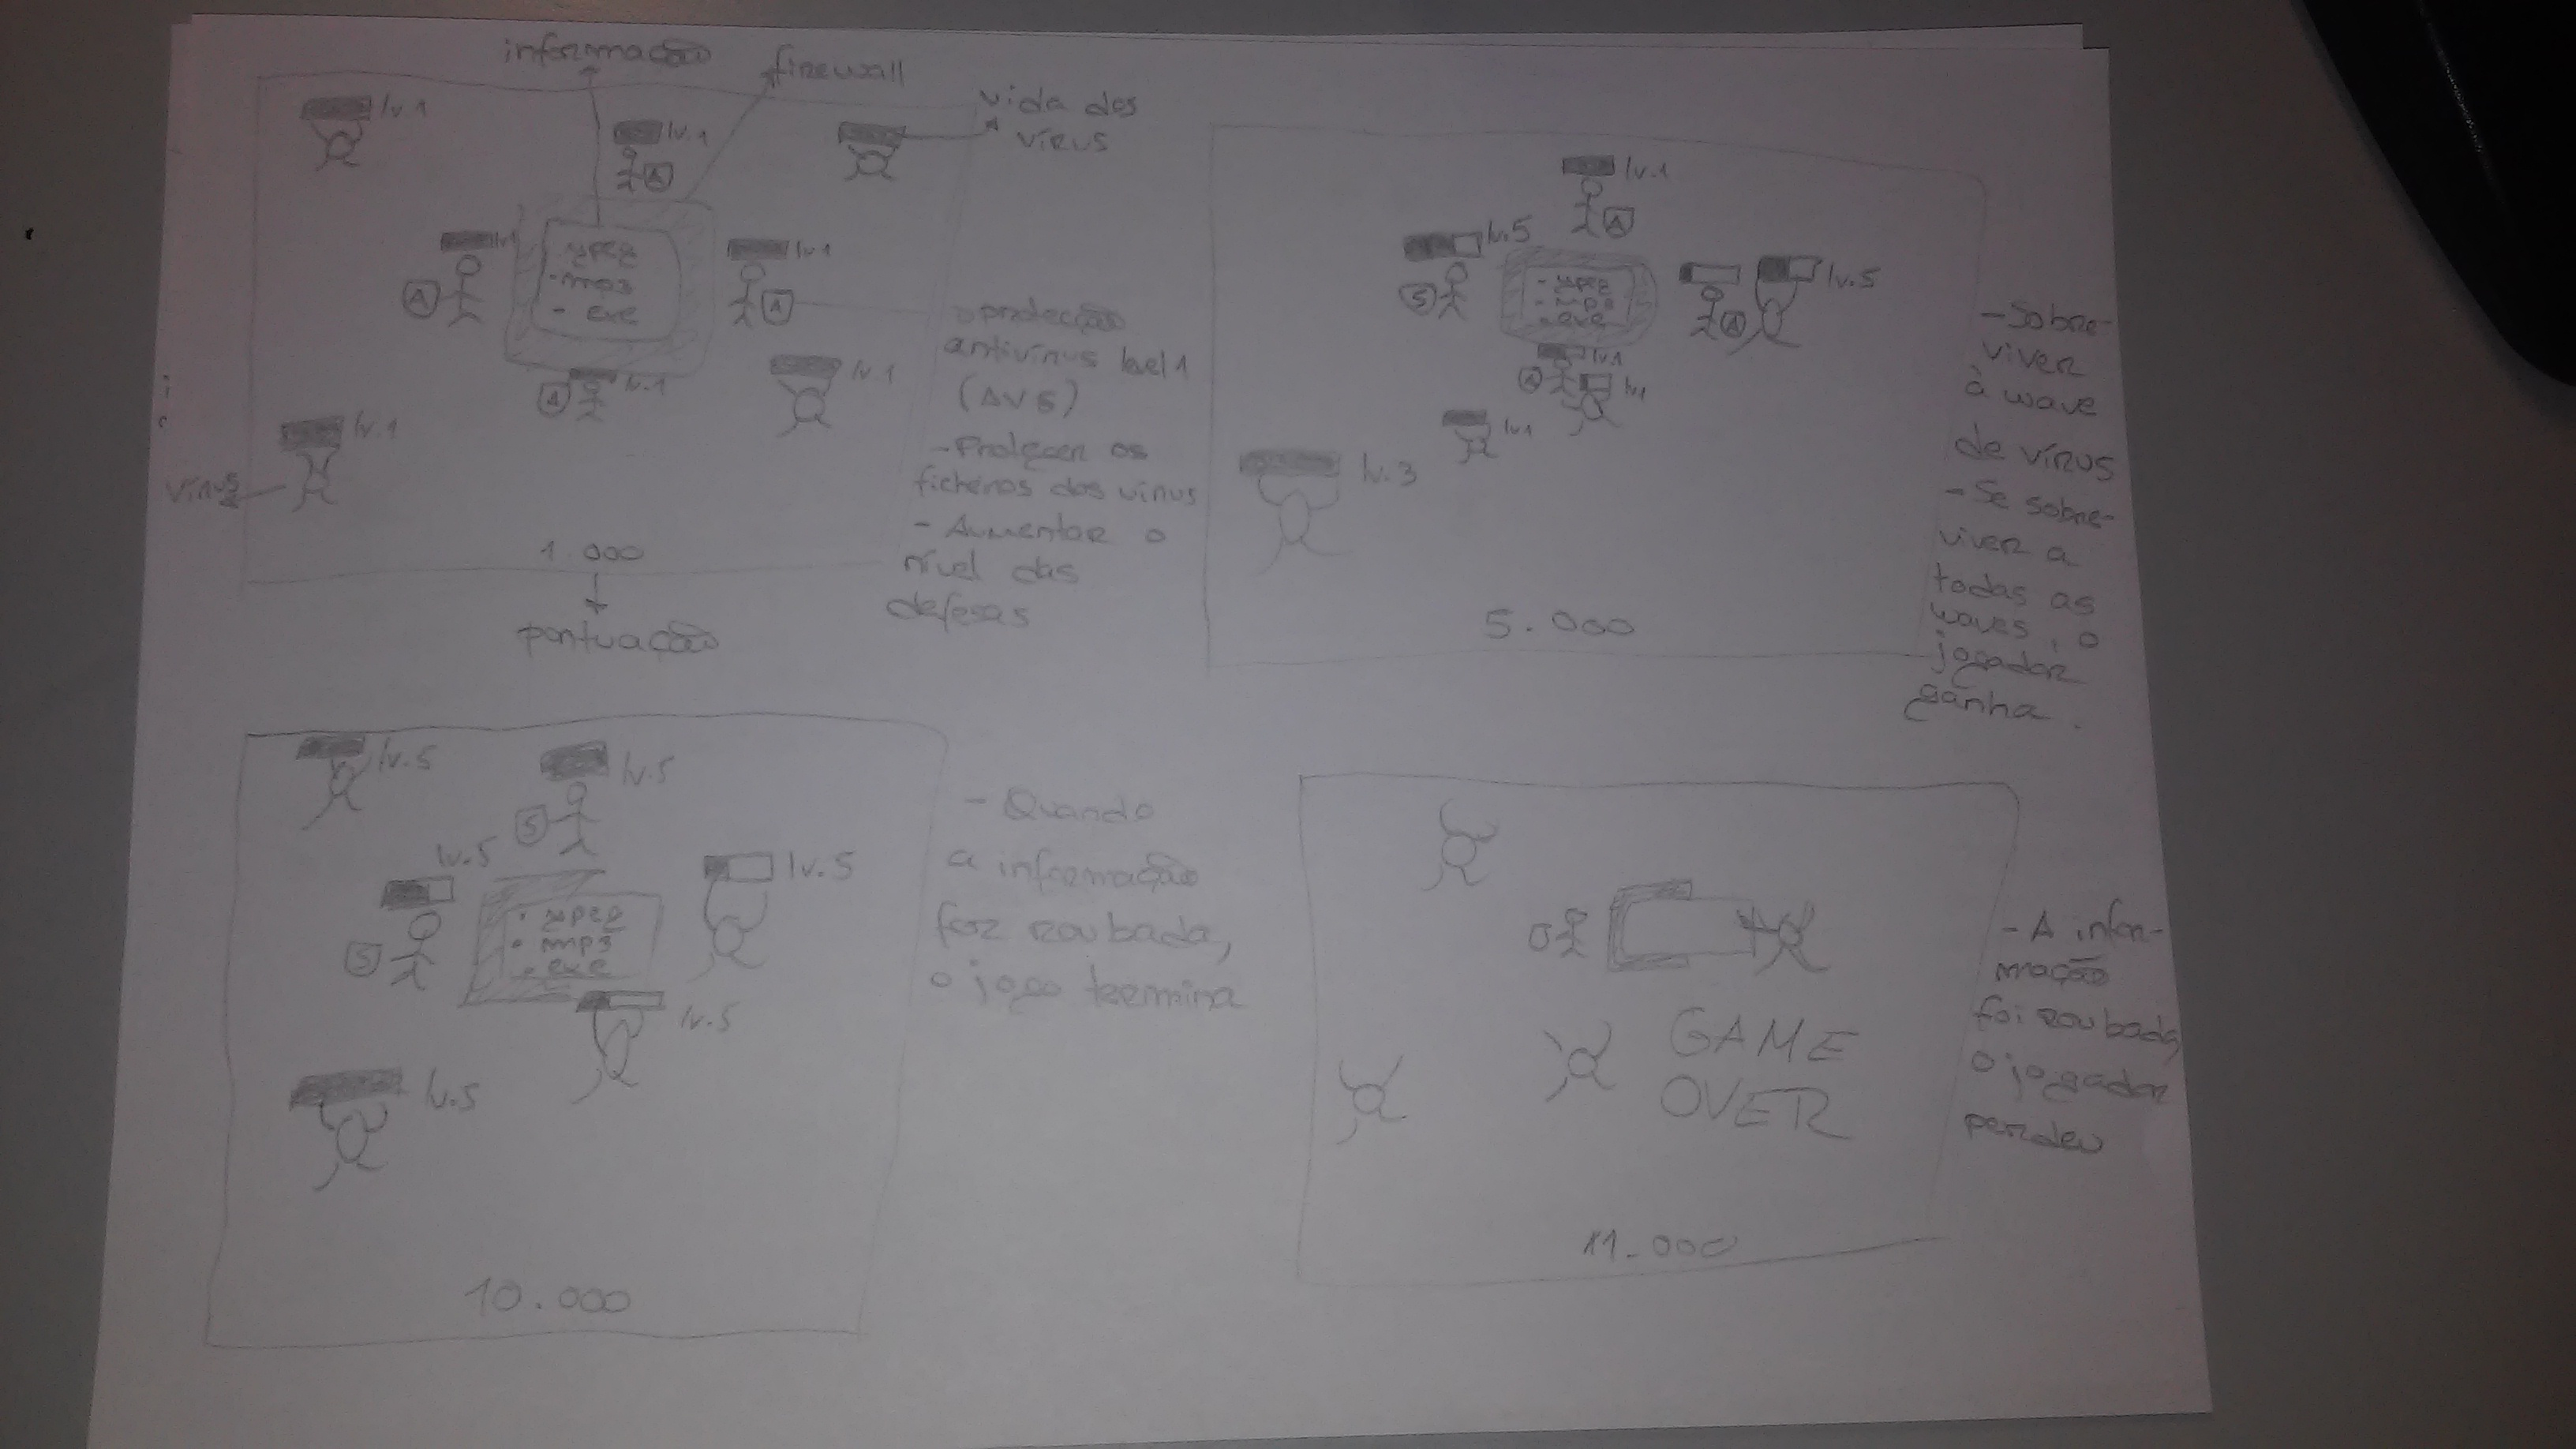
\includegraphics 
	[width = 0.75\textwidth] {Tiago/tiago_prototipo_1}
\caption{\label{att:fig:tiago:prot1}} Primeiro Protótipo do Tiago
\end{figure}

\begin{figure}[h]
\centering
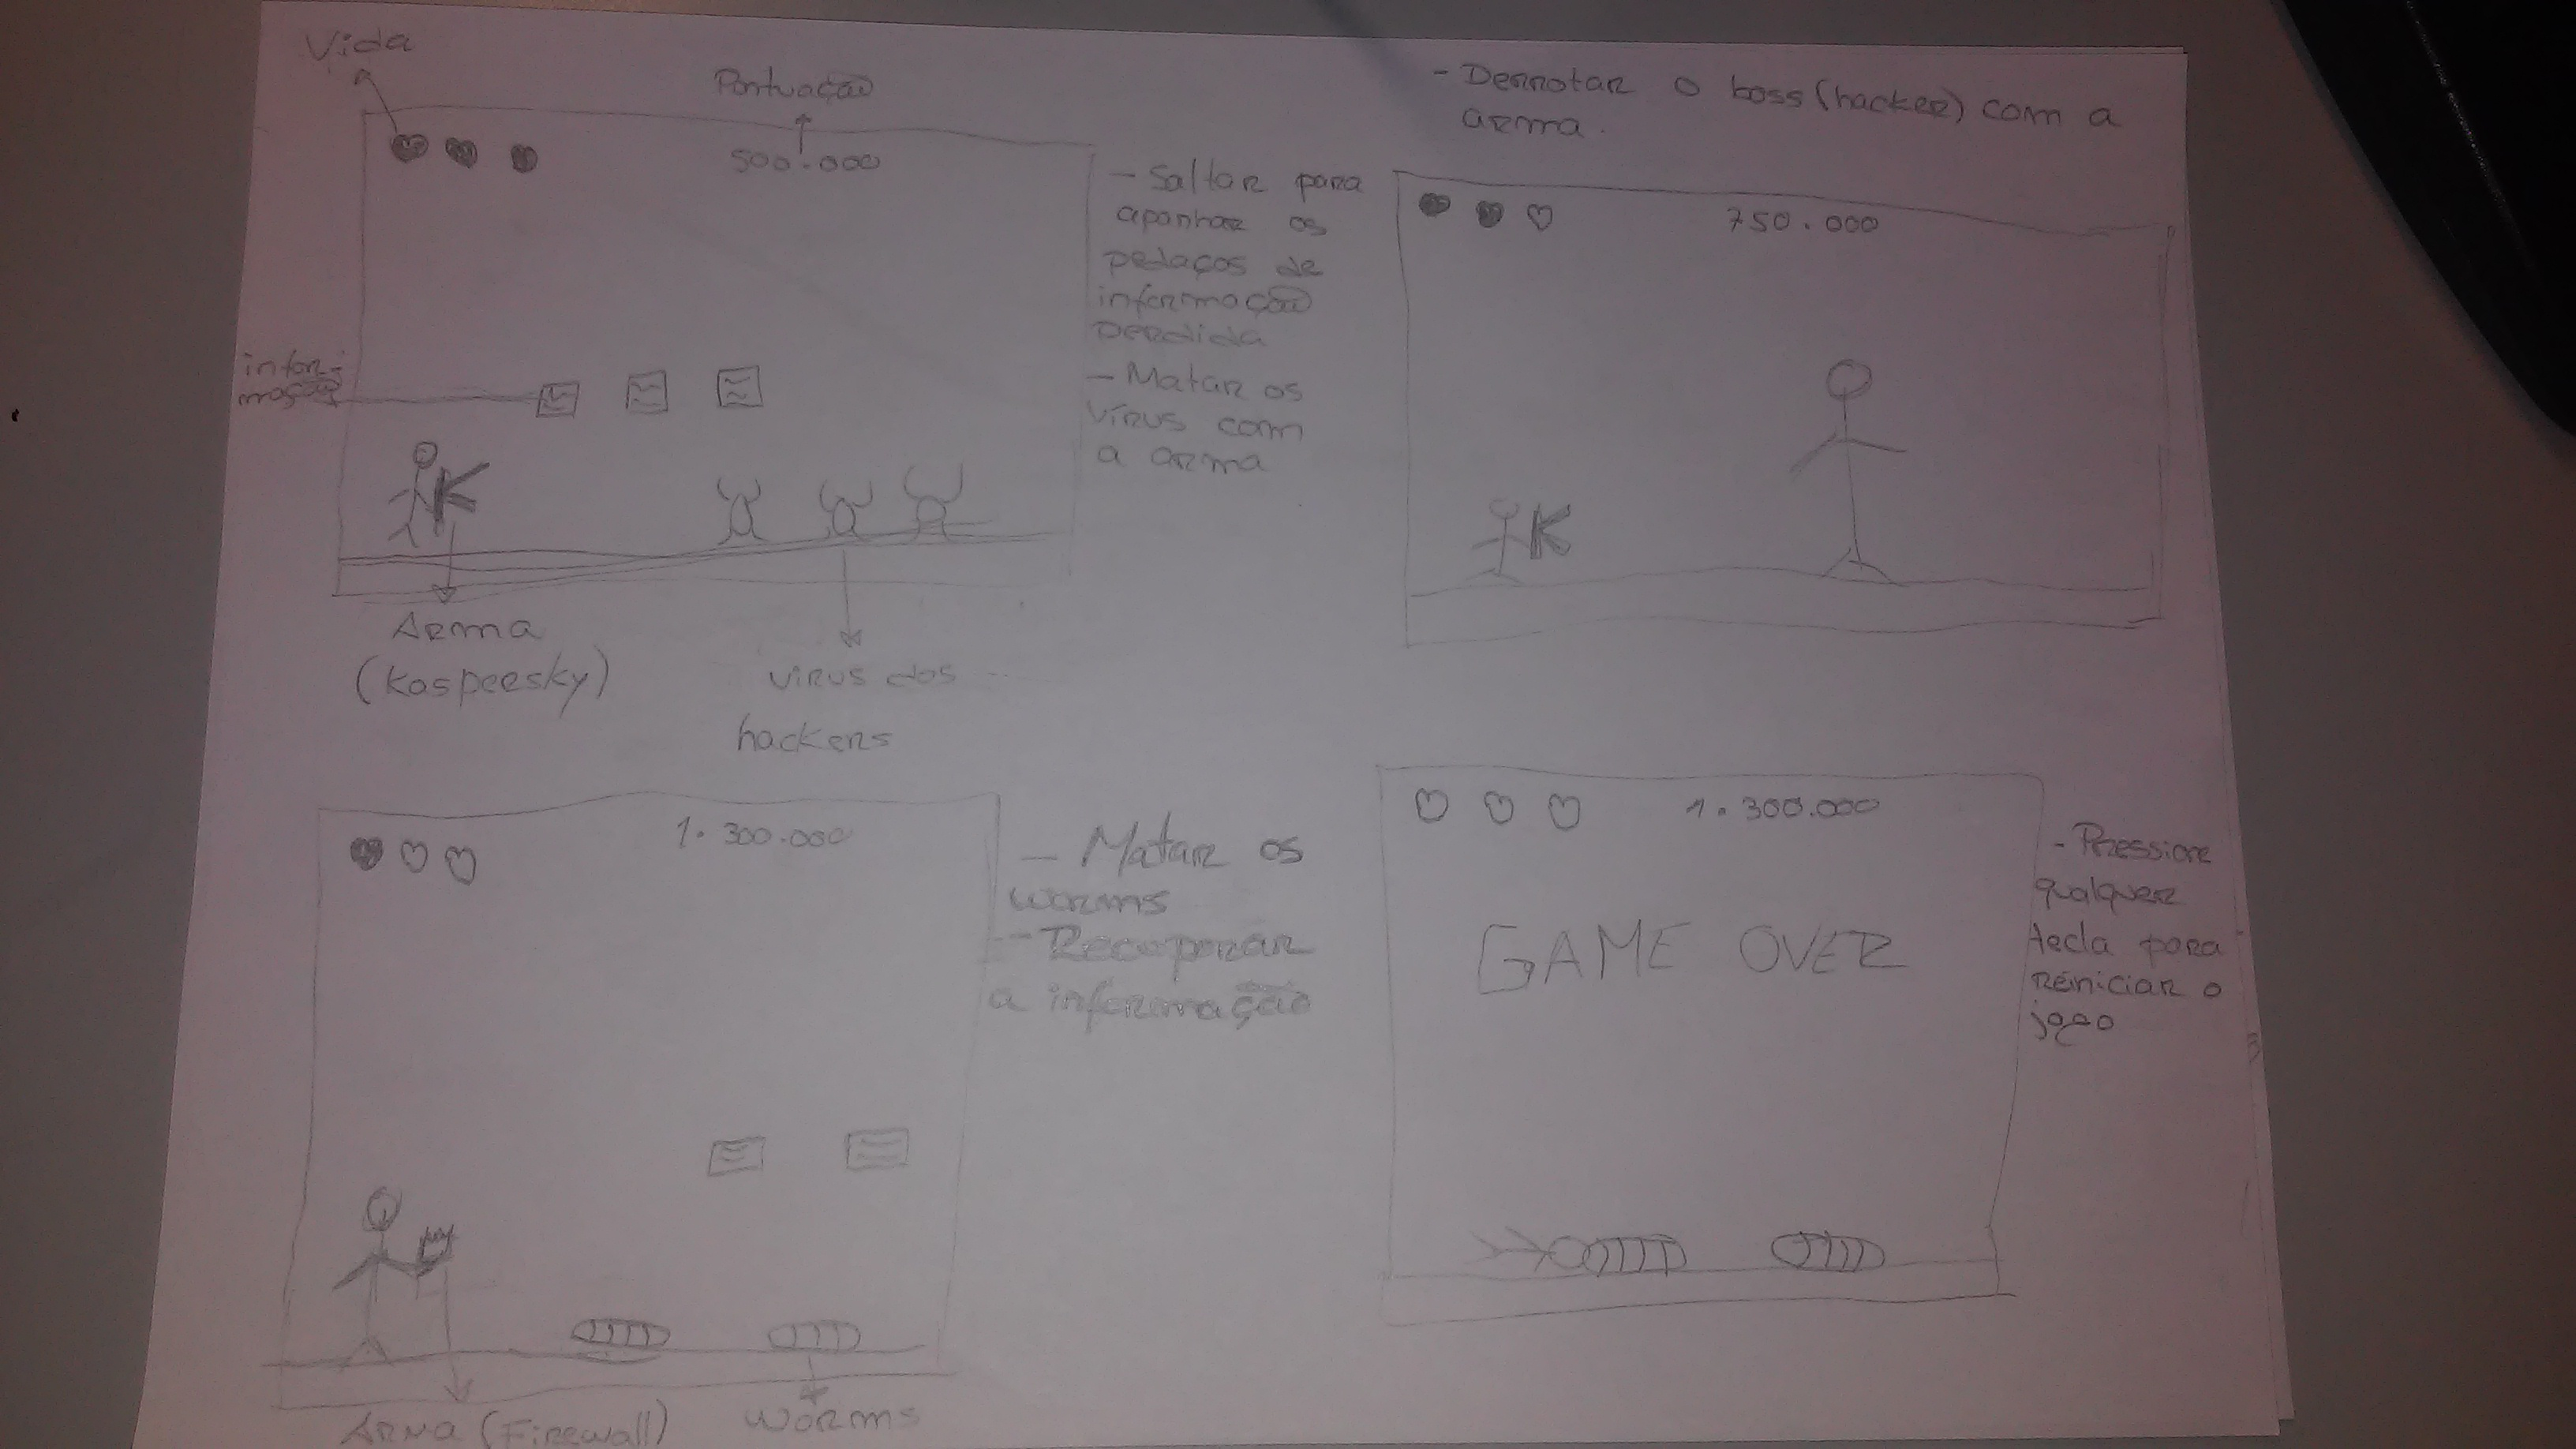
\includegraphics 
	[width = 0.75\textwidth] {Tiago/tiago_prototipo_2}
\caption{\label{att:fig:tiago:prot2}} Segundo Protótipo do Tiago
\end{figure}

\begin{figure}[h]
\centering
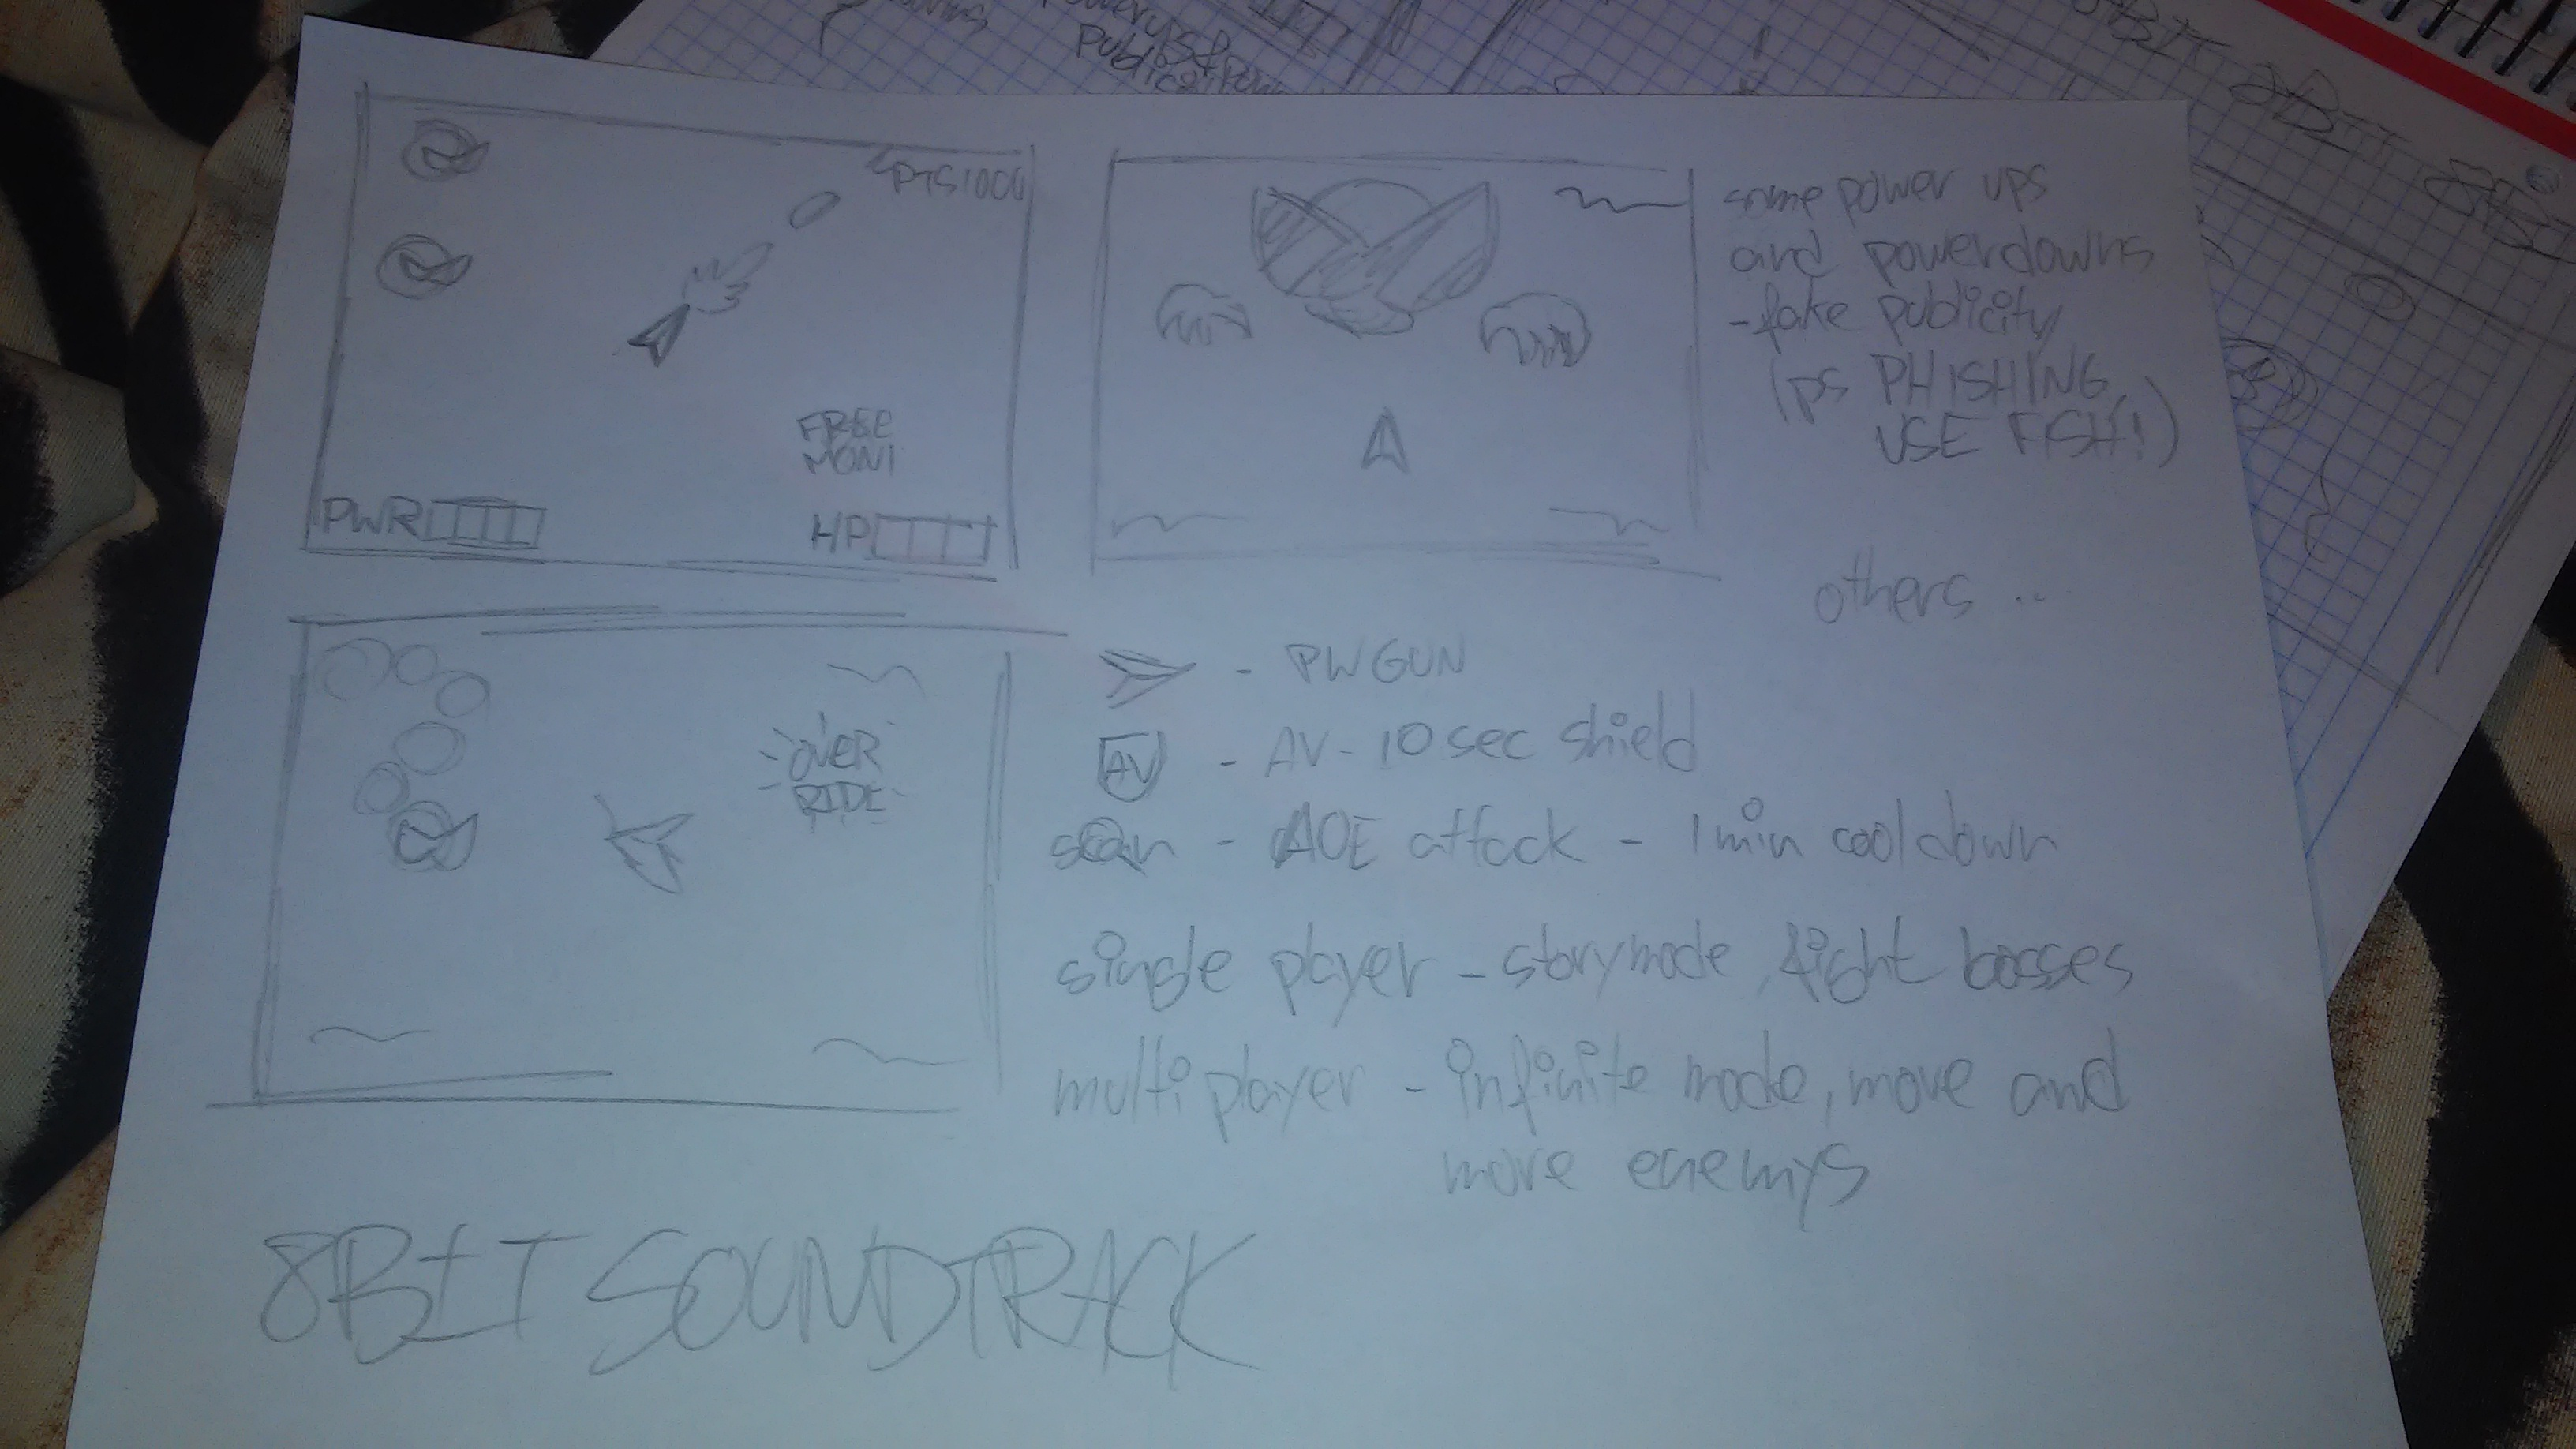
\includegraphics 
	[width = 0.75\textwidth] {Ian/ian_prototipo_1}
\caption{\label{att:fig:ian:prot1}} Primeiro Protótipo do Ian
\end{figure}

\begin{figure}[h]
\centering
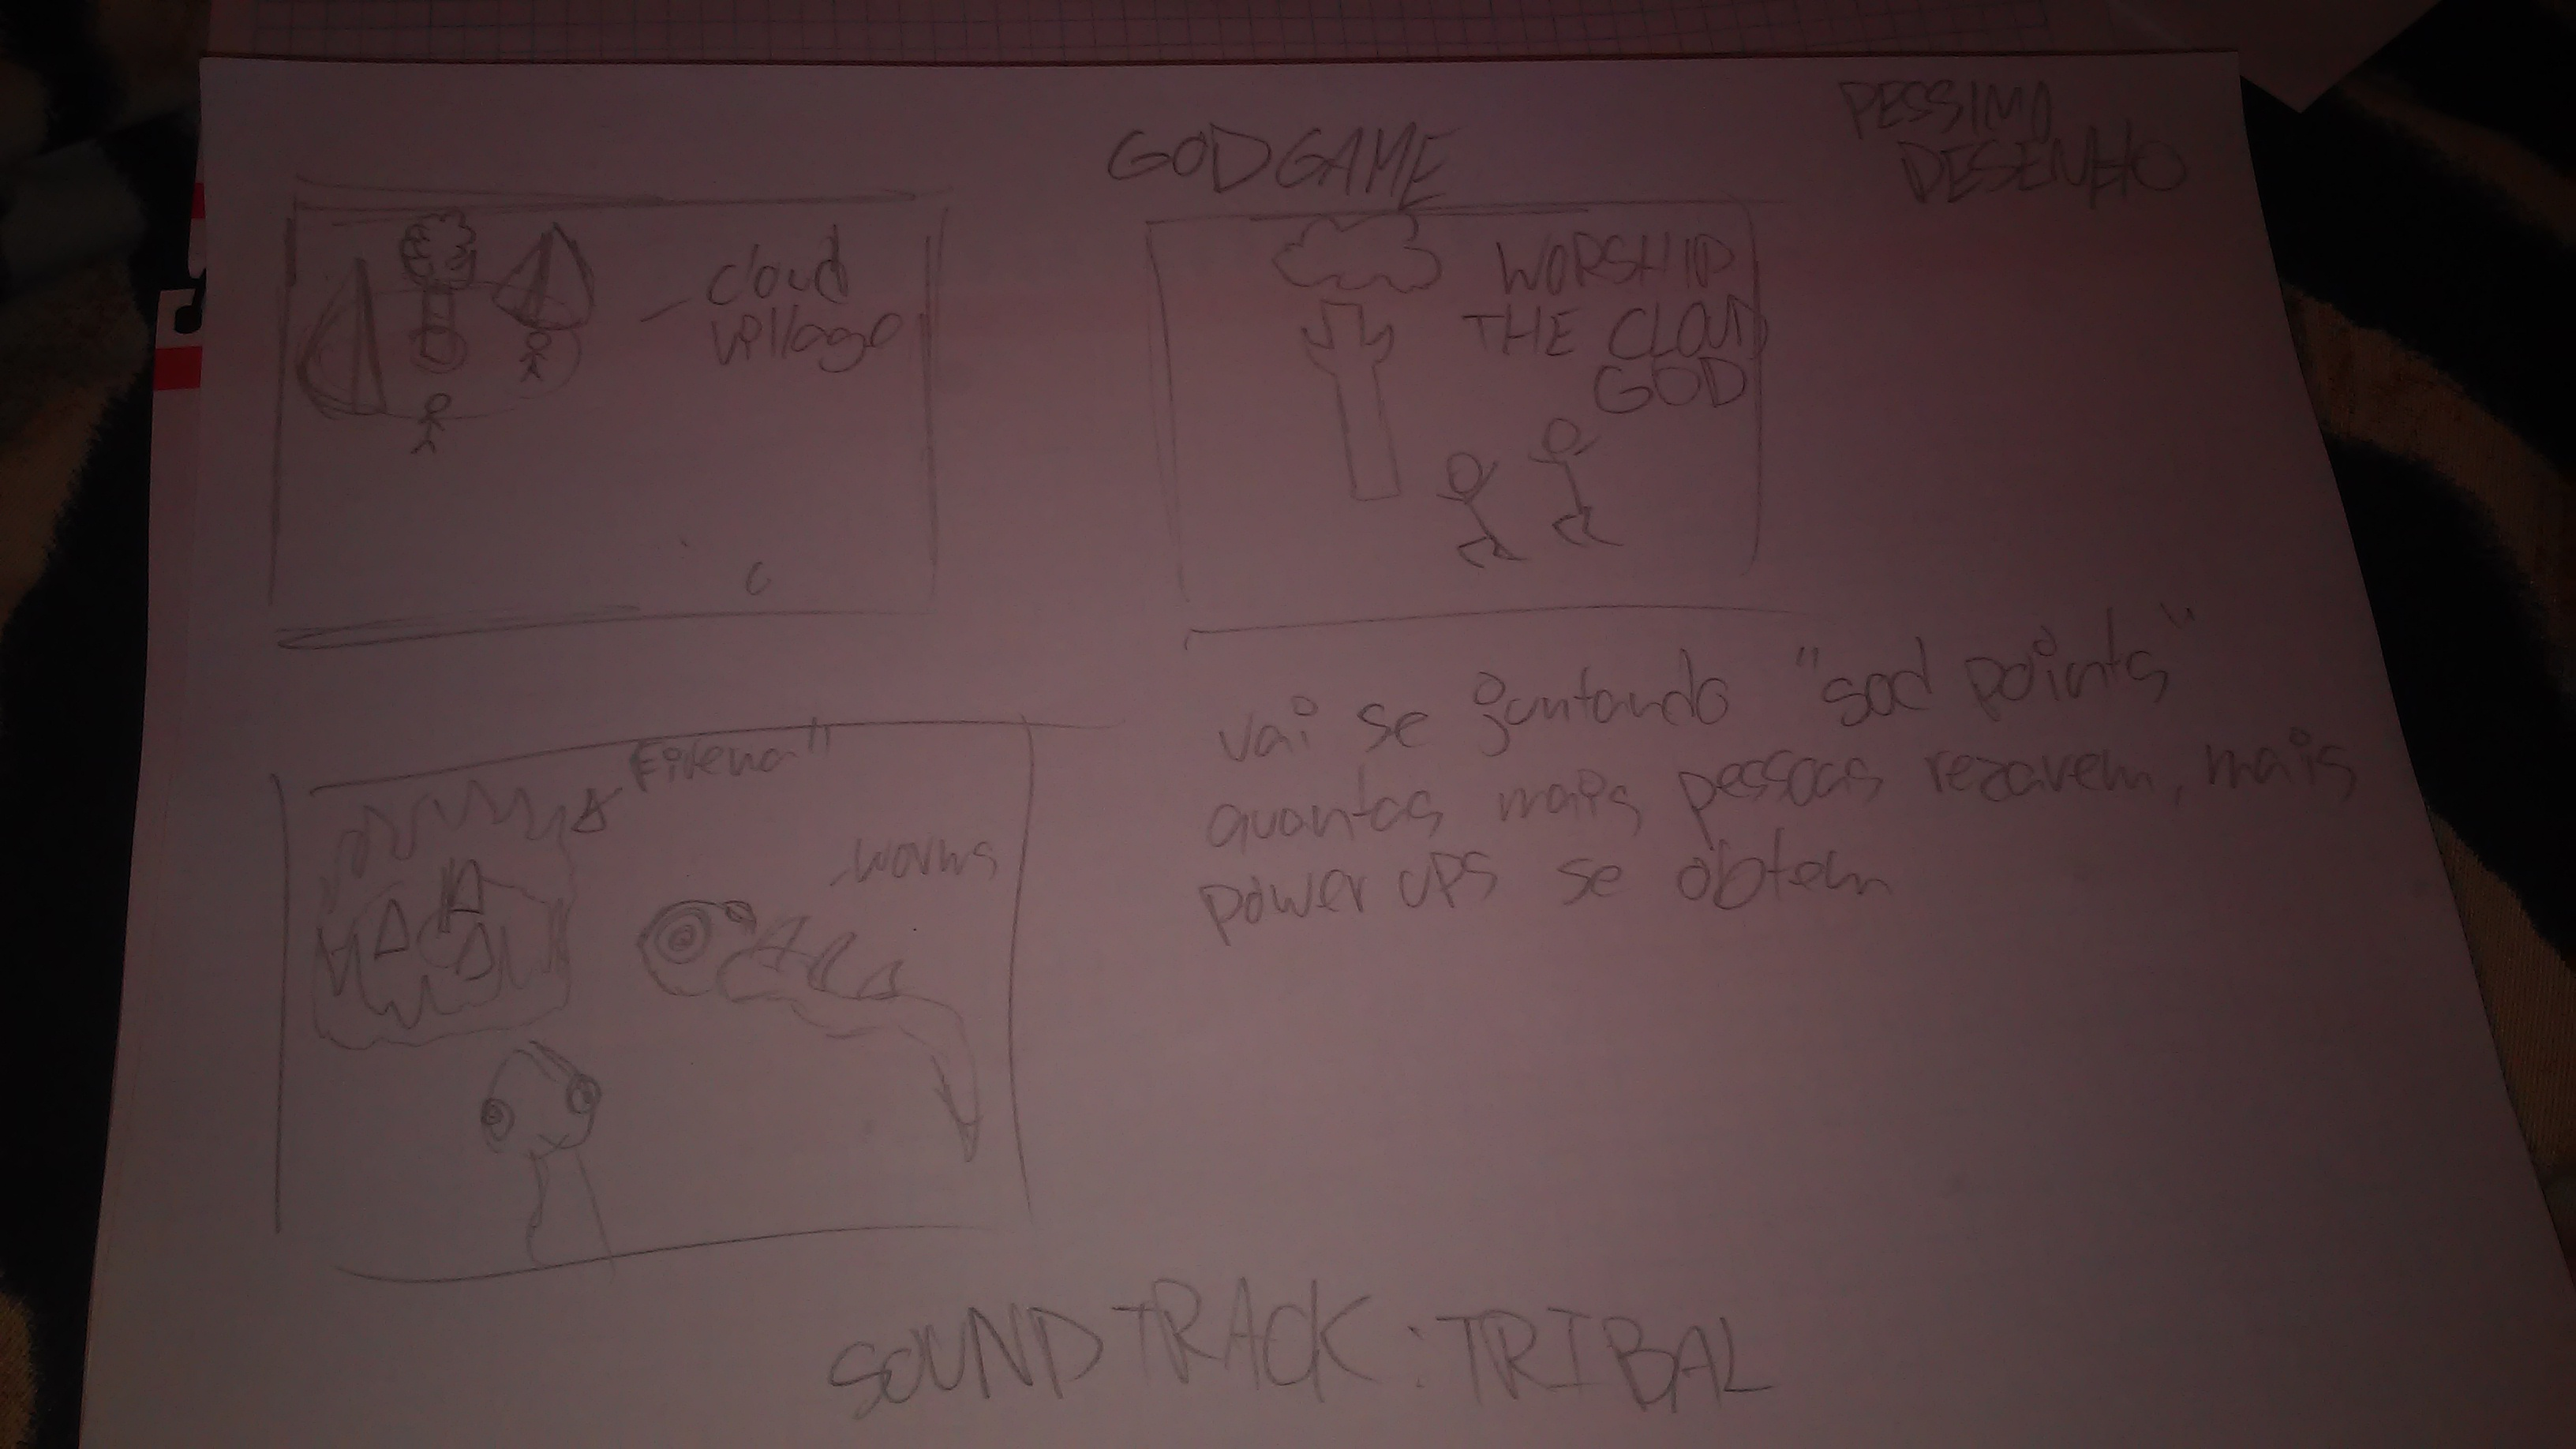
\includegraphics 
	[width = 0.75\textwidth] {Ian/ian_prototipo_2}
\caption{\label{att:fig:ian:prot2}} Segundo Protótipo do Ian
\end{figure}

\begin{figure}[h]
\centering
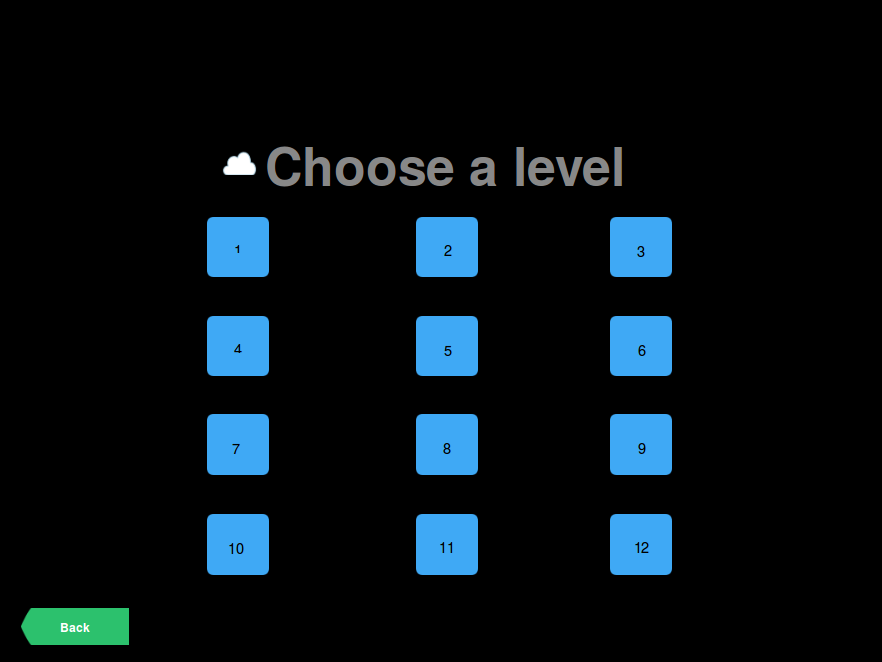
\includegraphics 
	[width = 0.65\textwidth] {FluiuiMenusPrototype}
\caption{\label{fig:fluidui}} Protótipo de Menus no FluidUI
\end{figure}

\begin{figure}[h]
\centering
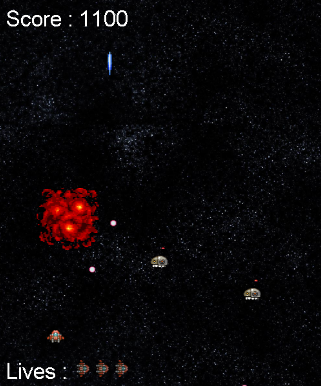
\includegraphics 
	[width = 0.65\textwidth] {PhaserGamePrototype}
\caption{\label{fig:phaser}} Protótipo de Jogo no Phaser
\end{figure}

\end{document}